\section{Introduction}\label{introduction}

Software maintenance activities such as debugging and feature
enhancement are known to be challenging and costly {[}@Pressman2005{]}.
Studies have shown that the cost of software maintenance can reach up to
70\% of the overall cost of the software development life cycle
{[}@HealthSocial2002{]}. Much of this is attributable to several factors
including the increase in software complexity, the lack of traceability
between the various artefacts of the software development process, the
lack of proper documentation, and the unavailability of the original
developers of the systems.

Research in software maintenance has evolved over the years to include
areas like mining bug repositories, bug analysis, prevention and
reproduction. The ultimate goal is to develop techniques and tools to
help software developers detect, correct, and prevent bugs in an
effective and efficient manner. Despite the recent advances in the
field, the literature shows that many existing software maintenance
tools have yet to be adopted by industry {[}@Lewis2013; @Foss2015;
@Layman2007; @Ayewah2007; @Ayewah2008; @Johnson2013; @Norman2013;
@Hovemeyer2004; @Lopez2011{]}. We believe that this is caused by the
following factors:

\begin{itemize}
\item
  Integration with the developer's workflow: Most existing maintenance
  tools ({[}@Kim2006a; @Ayewah2008b; @Findbugs2015; @Moha2010; @Palma;
  @Nayrolles2013d; @Nayrolles; @Nayrolles2013a; @Nayrolles2015a{]} are
  some noticeable examples) are not integrated well with the work flow
  of software developers (i.e., coding, testing, debugging, committing).
  Using these tools, developers have to download, install and understand
  them to achieve a given task. They would constantly need to switch
  from one workspace to another for different tasks (i.e., feature
  location with a command line tool, development and testing code with
  an IDE, development and testing front end code with another IDE and a
  browser, etc.){[}@Robertson2004; @Robertson2006; @Beckwith2006{]}.
\item
  Corrective actions: The outcome of these tools does not always lead to
  corrective actions that the developers can implement. Most of these
  tools return several results that are often difficult to interpret by
  developers. Take for example, FindBugs {[}@Hovemeyer2004{]}, a popular
  bug detection tool. This tool detects hundreds of bug signatures and
  reports them using an abbreviated code such as
  {CO\_COMPARETO\_INCORRECT\_FLOATING}. Using this code, developers can
  browse the FindBug's dictionary and find the corresponding definition
  {\emph{``This method compares double or float values using pattern
  like this: \(val1 > val2~?~1 : val1 < val2~?~-1 : 0\)''}}. While the
  detection of this bug pattern is accurate, the tool does not propose
  any corrective actions to the developers that can help them fix the
  problem. Moreover, it has been reported in the literature that the
  output of existing maintenance tools tends to be verbose at the point
  where developers decide to simply ignore them {[}@Arai2014; @Kim2007b;
  @Kim2007c; @Ayewah2010; @Shen2011{]}.
\item
  Leverage of historical data: These tools do not leverage a large body
  of knowledge that already exists in open source systems. For defect
  prevention, foe example, the state of the art approaches consists of
  adapting statistical models built for one project to another project
  {[}@Lo2013; @Nam2013{]}. As argued by Lewis {\emph{et al.}}
  {[}@Lewis2013{]} and Johnson {\emph{et al.}} {[}@Johnson2013{]},
  approaches based solely on statistical models are perceived by
  developers as black box solutions. Developers are less likely to trust
  the output of these tools.
\end{itemize}

In this thesis, we propose to address some of the above-mentioned issues
by focusing on developing techniques and tools that support software
maintainers at commit-time. As part of the developer's work flow, a
commit marks the end of a given task or subtask as the developer is
ready to version the source code. We propose a set of approaches in
which we intercept the commits and analyse them with the objective of
preventing unwanted modifications to the system. By doing so, we do not
only propose solutions that integrate well with the developer's work
flow, but also there is no need for software developers to use any other
external tools. As we will show in the rest of this proposal, some of
the techniques we propose rely on best practices found in a a large
repository of open source systems. In other words, we aim to leverage
historical data to guide new development efforts. We refer to the field
of study that encompasses software analysis techniques that operate on
code commits as software maintenance at commit-time.

More precisely, we propose the following contributions that we present
here and discuss in more detail in the next section:

\begin{itemize}
\item
  An aggregated bug repository system.
\item
  A clone prevention technique at commit-time.
\item
  A bug prevention technique at commit-time
\item
  A bug reproduction technique based on directed model checking and
  crash traces
\item
  A new classification of bugs based on the locations of the
  corrections.
\end{itemize}

\subsection{Research
Contributions{[}sec:objective-thesis{]}}\label{research-contributionssecobjective-thesis}

\subsubsection{An aggregate bug repository for developers and
researchers}\label{an-aggregate-bug-repository-for-developers-and-researchers}

When facing a new bug, one might want to leverage decades of open source
software history to find a suitable solution. The chances are that a
similar bug has already been fixed somewhere in another open source
project. The problem is that each open source project hosts its data in
a different data repository, using different bug tracking and version
control systems. Moreover, these systems have different interfaces to
access data. The data is not represented in a uniform way either. This
is further complicated by the fact that bug tracking tools and version
control systems are not necessarily connected. The former follows the
life of the bug, while the latter manages the fixes. As a result, one
would have to search the version control system repository to find
candidate solutions. Moreover, developers mainly use classical search
engines that index specialized sites such as StackOverflow. These sites
are organized in the form of question-response where a developer submits
a problem and receives answers from the community. While the answers are
often accurate and precise, they do not leverage the history of open
source software that has been shown to provide useful insights to help
with many maintenance activities such as bug fixing {[}@Saha2014{]}, bug
reproduction {[}@Nayrolles2015{]}, fault analysis {[}@Nessa2008{]}, etc.

In this work, we introduce BUMPER (BUg Metarepository for dEvelopers and
Researchers), a web-based infrastructure that can be used by software
developers and researchers to access data from diverse repositories
using natural language queries in a transparent manner, regardless of
where the data was originally created and hosted. The idea behind BUMPER
is that it can connect to any bug tracking and version control systems
and download the data into a single database. We created a common schema
that represents data, stored in various bug tracking and version control
systems. BUMPER uses a web-based interface to allow users to search the
aggregated database by expressing queries through a single point of
access. This way, users can focus on the analysis itself and not on the
way the data is represented or located. BUMPER supports many features
including: (1) the ability to use multiple bug tracking and control
version systems, (2) the ability to search very efficiently large data
repositories using both natural language and a specialized query
language, (3) the mapping between the bug reports and the fixes, and (4)
the ability to export the search results in Json, CSV and XML formats.

\subsubsection{An incremental approach for preventing bug and clone
insertion at commit
time}\label{an-incremental-approach-for-preventing-bug-and-clone-insertion-at-commit-time}

Code clones appear when developers reuse code with little to no
modification to the original code. Studies have shown that clones can
account for about 7\% to 50\% of code in a given software system
{[}@Baker; @StephaneDucasse{]}. Developers often reuse code (and create
clones) in their software on purpose {[}@Kim2005{]}. Nevertheless,
clones are considered a bad practice in software development since they
can introduce new bugs in the code {[}@Kapser2006; @Juergens2009;
@Li2006{]}. If a bug is discovered in one segment of the code that has
been copied and pasted several times, then the developers will have to
remember the places where this segment has been reused in order to fix
the bug in each place. In the last two decades, there have been many
studies and tools that aim at detecting clones. They can be grouped into
three categories. Although these techniques and tools have been shown to
be useful in detecting clones, they operate in an off-line fashion
(i.e., after the clones have been inserted). Software developers might
be reluctant to use these tools on a day-today basis (i.e., as part of
the continuous development process), unless they are involved in a major
refactoring effort. This problem is somehow similar to the problem of
adopting bug identification tools. Johnson et al. {[}@Johnson2013{]}
showed that these tools are challenging to use because they do not
integrate well with the day-to-day work flow of a developer. Also they
output a large amount of data when applied to the entire system, making
it hard to understand and analyse their results.

In this research, we present PRECINCT (PREventing Clones INsertion at
Commit Time) that focuses on preventing the insertion of clones at
commit time, i.e., before they reach the central code repository.
PRECINCT is an online clone detection technique that relies on the use
of pre-commit hooks capabilities of modern source code version control
systems. A pre-commit hook is a process that one can implement to
receive the latest modification to the source code done by a given
developer just before the code reaches the central repository. PRECINCT
intercepts this modification and analyses its content to see whether a
suspicious clone has been introduced or not. A flag is raised if a code
fragment is suspected to be a clone of an existing code segment. In
fact, PRECINCT, itself, can be seen as a pre-commit hook that detects
clones that might have been inserted in the latest changes with regard
to the rest of the source code.

Similar to clone detection, we propose an approach for preventing the
introduction of bugs at commit-time. Many tools exist to prevent a
developer to ship {\emph{bad}} code {[}@Dangel2000; @Hovemeyer2007;
@Moha2010{]} or to identify {\emph{bad}} code after executions (e.g in
test or production environment) {[}@Nayrolles; @Nayrolles2013a{]}.
However, these tools rely on metrics and rules to statically and/or
dynamically identify sub-optimum code. Our approach, called {BIANCA}
(Bug Insertion ANticipation by Clone Analysis at merge time), is
different than the approaches presented in the literature because it
mines and analyses the change patterns in commits and matches them
against past commits known to have introduced a defect in the code (or
that have just been replaced by better implementation).

\subsubsection{A bug reproduction technique based on a combination of
crash traces and model
checking}\label{a-bug-reproduction-technique-based-on-a-combination-of-crash-traces-and-model-checking}

When a system crashes, software developers need to reproduce the crash
(usually in a lab environment) so as to provide corrective measures. A
survey conducted with the developers of major open source software
systems such as Apache, Mozilla and Eclipse revealed that one of the
most valuable piece of information that can help locate and fix the
cause of a crash is the one that can help reproduce it
{[}@Bettenburg2008{]}. Crash reproduction is an expensive task because
the data provided by end users is often scarce {[}@Artzi2008; @Jin2012;
@Chen2013{]}. It is therefore important to invest in techniques and
tools for automatic bug reproduction to ease the maintenance process and
accelerate the rate of bug fixes and patches. Existing techniques can be
divided into two categories: (a) On-field record and in-house replay
{[}@Steven2000; @Narayanasamy2005; @Artzi2008; @Roehm2015{]}, and (b)
In-house crash explanation {[}@Jin2012; @Jin2013; @Zuddas2014;
@Chen2013a; @Nayrolles2015{]}.

In this work, we propose an approach, called JCHARMING (Java CrasH
Automatic Reproduction by directed Model checkING) that uses a
combination of crash traces and model checking to automatically
reproduce bugs that caused field failures. Unlike existing techniques,
JCHARMING does not require instrumentation of the code. It does not need
access to the content of the heap either. Instead, JCHARMING uses a list
of functions output when an uncaught exception in Java occurs (i.e., the
crash trace) to guide a model checking engine to uncover the statements
that caused the crash.

\subsubsection{A new taxonomy of bugs based on the locations of the
corrections --- an empirical
Study}\label{a-new-taxonomy-of-bugs-based-on-the-locations-of-the-corrections-an-empirical-study}

There have been several studies (e.g., {[}@Weiß2007; @Zhang2013{]}) that
study of the factors that influence the bug fixing time. These studies
empirically investigate the relationship between bug report attributes
(description, severity, etc.) and the fixing time. Other studies take
bug analysis to another level by investigating techniques and tools for
bug prediction and reproduction (e.g., {[}@Chen2013; @Kim2007a;
@Nayrolles2015{]}). These studies, however, treat all bugs as the same.
For example, a bug that requires only one fix is analysed the same way
as a bug that necessitates multiple fixes. Similarly, if multiple bugs
are fixed by modifying the exact same locations in the code, then we
should investigate how these bugs are related in order to predict them
in the future. Note here that we do not refer to duplicate bugs.
Duplicate bugs are marked as duplicate (and not fixed) and only the
master bug is fixed. From the bug handling perspective, if we can
develop a way to detect related bug reports during triaging then we can
achieve considerable time saving in the way bug reports are processed,
for example, by assigning them to the same developers.We also conjecture
that detecting related bugs can help with other tasks such as bug
reproduction. We can reuse the reproduction of an already fixed bug to
reproduce an incoming and related bug.

We investigate the relationship between bugs by examining their
locations of the fixes. By a fix, we mean a modification (adding or
deleting lines of code) to an exiting file that is used to solve the
bug.We argue that bugs can be classified into four types: A bug of Type
1 refers to a bug being fixed in one single location (i.e., one file),
while Type 2 refers to bugs being fixed in more than one location. Type
3 refers to multiple bugs that are fixed in the exact same location.
Type 4 is an extension of Type 3, where multiple bugs are resolved by
modifying the same set of locations. Note that Type 3 and Type 4 bugs
are not duplicates, they may occur when different features of the system
fail due to the same root causes (faults). We conjecture that knowing
the proportions of each type of bugs in a system may provide insights
into the quality of the system. Knowing, for example, that in a given
system the proportion of Type 2 and 4 bugs is high may be an indication
of poor system quality since many fixes are needed to address these
bugs. In addition, the existence of a high number of Types 3 and 4 bugs
calls for techniques that can effectively find bug reports related to an
incoming bug during triaging. This is similar to the many studies that
exist on detection of duplicates (e.g., {[}@Runeson2007; @Sun2010;
@Nguyen2012{]}), except that we are not looking for duplicates but for
related bugs (bugs that are due to failures of different features of the
system, caused by the same faults).

\subsection{Outline{[}sec:outline{]}}\label{outlinesecoutline}

The remaining chapters of this proposal are:

\begin{itemize}
\item
  Chapter {[}chap:relwork{]} - {\emph{Background \& Related work}}. In
  this chapter, we present the major studies related to our research
  field, namely, crash reproduction, aggregating bug repositories for
  mining purposes, and clone detection.
\item
  Chapter {[}chap:bumper{]} - {\emph{An Aggregate Bug Repository for
  Developers and Researchers}}. In this chapter, we present {BUMPER}
  (BUg Metarepository for dEvelopers and Researchers), our bug
  meta-repository. {BUMPER} acts as our data source for the different
  contributions.
\item
  Chapter {[}chap:jcharming{]} - {\emph{JCHARMING: Java CrasH Automatic
  Reproduction by directed Model checkING}}. In this chapter we discuss
  the components of JCHARMING, the bug reproduction approach we propose.
\item
  Chapter {[}chap:clone-detection-pragmatic{]} - {\emph{Preventing Clone
  Insertion}}. This chapter describes one approach to prevent the
  insertion of clones at commit time.
\item
  Chapter {[}chap:bianca{]} - {\emph{Preventing Bug Insertion Using
  Clone Detection}}. In this chapter, we present an approach named
  {BIANCA} (Bug Insertion ANticipation by Clone Analysis at merge time)
  which uses clone detection to prevent bug insertion.
\item
  Chapter {[}chap:plan{]} - {\emph{Remaining Work}} presents the
  remaining work and a publication plan.
\end{itemize}

\section{Background \& Related
Work{[}chap:relwork{]}}\label{background-related-workchaprelwork}

In this chapter we present background in Section
{[}sec:preliminaries{]}. We define key concepts using throughout this
proposal. Then, we present related work for bug reproduction, bug
prediction, and clone detection.

\subsection{Preliminaries{[}sec:preliminaries{]}}\label{preliminariessecpreliminaries}

\subsubsection{Definitions{[}sec:version-control{]}}\label{definitionssecversion-control}

In this proposal, we use the following definitions that are based on
{[}@Avizienis2004; @Pratt2001; @Burnstein2006; @Radatz1990;
@Whittaker2012{]}.

\begin{itemize}
\item
  Software bug: A software bug is an error, flaw, failure, defect or
  fault in a computer program or system that causes it to violate at
  least one of its functional or non-functional requirement.
\item
  Error: An error is a mistake, misconception, or misunderstanding on
  the part of a software developer.
\item
  Fault/defect: A fault (defect) is defined as an abnormal condition or
  defect at the component, equipment, or subsystem level which may lead
  to a failure. A fault (defect) is not final (the system still works)
  and does not prevent a given feature to be accomplished. A fault
  (defect) is a deviation (anomaly) of the healthy system that can be
  caused by an error or external factors (hardware, third parties,
  etc.).
\item
  Failure: The inability of a software system or component to perform
  its required functions within specified requirements.
\item
  Crash: The software system encountered a fault (defect) that triggered
  a fatal failure from which the system could not recover from/overcome.
  As a result, the system stops.
\item
  Bug report: A bug report describes a behaviour observed in the field
  and considered abnormal by the reporter. Bug reports are submitted
  manually to bug report systems (bugzilla/jira). There is no mandatory
  format to report a bug. Nevertheless, a bug report should have: the
  version of the software system, OS, and platform, steps to reproduce
  the bug, screen shots, stack trace and anything that could help a
  developer assess the internal state of the software system.
\item
  Crash report: A crash report is issued as the last thing that a
  software system does before crashing. Crash reports are usually
  reported automatically (crash reporting systems are implemented as
  part of the software). A crash report contains data (that can be
  proprietary) to help developers understand the causes of the crash
  (e.g., memory dump,\ldots{}).
\end{itemize}

In the remaining of this section, we introduce the two types of software
repositories: version control and project tracking system.

\subsubsection{Version control
systems{[}sec:version-control{]}}\label{version-control-systemssecversion-control}

Version control consists of maintaining the versions of various
artefacts such as source code files {[}@Zeller1997{]}. This activity is
a complex task and cannot be performed manually in real world projects.
To this end, there exist several tools that have been created to help
practitioners manage the version of their software artefacts. Each
evolution of a software system is considered as a version (also called
revision) and each version is linked to the one before through
modifications of software artefacts. These modifications consist of
updating, adding or deleting software artefacts. They can be referred as
\texttt{diff}, {patch} or {commit}\footnote{The bug reports used in this
  study and the result of the model checker are made available for
  download from research.mathieu- nayrolles.com/jcharming/ In order to
  classify the research on the different fields related to software
  maintenance, we can reason about types of bugs at different levels.
  For example, we can group bugs based on the developers that fix them
  or using information about the bugs such as crash traces.}. A
\texttt{diff}, {patch} or {commit} has the following characteristics:

\begin{itemize}
\item
  Number of files: The number of software files that have been modified,
  added or deleted.
\item
  Number of hunks: The number of consecutive code blocks of modified,
  added or deleted lines in textual files. Hunks are used to determine,
  in each file, how many different places the developer has modified.
\item
  Number of churns: The number of modified lines. However, the churn
  value for a line change should be at least two as the line has to be
  deleted first and then added back with the modifications.
\end{itemize}

Modern version control systems also support branching. A branch is a
derivation in the evolution that contains a duplication of the source
code so that both versions can be modified in parallel. Branches can be
reconciled with a merge operation that merge modifications of two or
more branches. This operation is completely automated at the exception
of merging conflicts that arise when both branches contain modifications
of the same line. Such conflicts cannot be reconciled automatically and
have to be dealt with by the developers. This allows for a greater
agility among developers as changes in one branch do not affect the work
of the developers that is on other branches.

Branching has been used for more than testing hazardous refactoring or
testing framework upgrades. Task branching is an agile branching
strategy where a new branch is created for each task
{[}@MartinFowler2009{]}. It is common to see a branch named
{123\_implement\_X} where {123} is the {\#id} of task {X} given by the
project tracking system. Project tracking systems are presented in
Section {[}sec:issue-tracking{]}.

In modern versioning systems, when maintainers make modifications to the
source code, they have to commit their changes for the modifications to
be effective. The commit operation versions the modifications applied to
one or many files.

Figure {[}fig:branching{]} presents the data structure used to store a
commit. Each commit is represented as a tree. The root leaf (green)
contains the commit, tree and parent hashes as same as the author and
the description associated with the commit. The second leaf (blue)
contains the leaf hash and the hashes of the files of the project.

\begin{figure}[htbp]
\centering
\includegraphics{media/commit-datastructure.png}
\caption{Data structure of a commit. {[}fig:branching{]}}
\end{figure}

In this example, we can see that author ``Mathieu'' has created the file
\(file1.java\) with the message ``project init''. Figure
{[}fig:two-commits{]} represents an external modification. In this
second example, \(file1. java\) is modified while \(file2.java\) is
created. The second commit \(98ca9\) have \(34ac2\) as a parent.

\begin{figure}[htbp]
\centering
\includegraphics{media/branching.png}
\caption{Data structure of two commits. {[}fig:two-commits{]}}
\end{figure}

Branches point to a commit. In a task-branching environment, a branch is
created via a checkout operation for each task. Tasks can be to fix the
root cause of a crash or bug report or features to implement. In figure
{[}fig:two-branches{]}, the \(master\) branch and the
\(1\_fix\_overflow\) point on commit \(98ca9\).

\begin{figure}[htbp]
\centering
\includegraphics{media/2branches.png}
\caption{Two branches pointing on one commit. {[}fig:two-branches{]}}
\end{figure}

Both branches can evolve separately and be merged together when the task
branch is ready. In Figure {[}fig:merge{]}, the \(master\) branch points
on \(a13ab2\) while the \(1\_fix\_overflow\) points on \(ahj23k\).

\begin{figure}[htbp]
\centering
\includegraphics{media/merge.png}
\caption{Two branches pointing on two commits. {[}fig:merge{]}}
\end{figure}

\paragraph{Providers{[}sec:revision-provider{]}}\label{providerssecrevision-provider}

In this proposal, we mainly refer to three version control systems:
{Svn}, {Git} and, to a lesser extent, {Mercurial}. {SVN} is distributed
by the Apache Foundation and is a centralized concurrent version system
that can handle conflicts in the different versions of different
developers. SVN is widely used in industry. At the opposite, {Git} is a
distributed revision control system --- originally developed by Linus
Torvald --- where revisions can be kept locally for a while and then
shared with the rest of the team. Finally, {Mercurial} is also a
distributed revision system, but shares a lot of concepts with {SVN}. It
will be easier for people who are used to {SVN} to switch to a
distributed revision system if they use {Mercurial}.

\subsubsection{Project Tracking
Systems{[}sec:issue-tracking{]}}\label{project-tracking-systemssecissue-tracking}

Project tracking systems allow end users to create bug reports (BRs) to
report unexpected system behaviour, managers can create tasks to drive
the evolution forward and crash report (CRs) can be automatically
created. These systems are also used by development teams to keep track
of the modifications induced by bug and to crash reports, and keep track
of the fixes.

\begin{figure}[htbp]
\centering
\includegraphics{media/bzLifecycle.png}
\caption{Lifecyle of a report {[}@Bugzilla2008{]}{}}
\end{figure}

Figure {[}fig:bug-lifecyle{]} presents the life cycle of a report. When
a report is submitted by an end-user, it is set to the {UNCONFIRMED}
state until it receives enough votes or that a user with the proper
permissions modifies its status to {NEW}. The report is then assigned to
a developer to be fixed. When the report is in the {ASSIGNED} state, the
assigned developer(s) starts working on the report. A fixed report moves
to the {RESOLVED} state. Developers have five different possibilities to
resolve a report: {FIXED}, {DUPLICATE}, {WONTFIX}, {WORKSFORME} and
{INVALID} {[}@Koponen2006{]}.

\begin{itemize}
\item
  {RESOLVED/FIXED}: A modification to the source code has been pushed,
  i.e., a changeset (also called a patch) has been committed to the
  source code management system and fixes the root problem described in
  the report.
\item
  {RESOLVED/DUPLICATE}: A previously submitted report is being
  processed. The report is marked as duplicate of the original report.
\item
  {RESOLVED/WONTFIX}: This is applied in the case where developers
  decide that a given report will not be fixed.
\item
  {RESOLVED/WORKSFORME}: If the root problem described in the report
  cannot be reproduced on the reported OS / hardware.
\item
  {RESOLVED/INVALID}: If the report is not related to the software
  itself.
\end{itemize}

Finally, the report is {CLOSED} after it is resolved. A report can be
reopened (sent to the {REOPENED} state) and then assigned again if the
initial fix was not adequate (the fix did not resolve the problem). The
elapsed time between the report marked as the new one and the resolved
status are known as the {\emph{fixing time}}, usually in days. In case
of task branching, the branch associated with the report is marked as
ready to be merged. Then, the person in charge (quality assurance team,
manager, ect\ldots{}) will be able to merge the branch with the
mainline. If the report is reopened: the days between the time the
report is reopened and the time it is marked again as {RESOLVED/FIXED}
are cumulated. Reports can be reopened many times.

Tasks follow a similar life cycle with the exception of the
{UNCONFIRMED} and {RESOLVED} states. Tasks are created by management and
do not need to be confirmed in order to be {OPEN} and {ASSIGNED} to
developers. When a task is complete, it will not go to the {RESOLVED}
state, but to the {IMPLEMENTED} state. Bug and crash reports are
considered as problems to eradicate in the program. Tasks are considered
as new features or amelioration to include in the program.

Reports and tasks can have a severity associated to
them{[}@Bettenburg2008{]}. The severity indicates the degree of impact
on the software system. The possible severities are:

\begin{itemize}
\item
  blocker: blocks development and/or testing work.
\item
  critical: crashes, loss of data, severe memory leak.
\item
  major: major loss of function.
\item
  normal: regular report, some loss of functionality under specific
  circumstances.
\item
  minor: minor loss of function, or other problem where easy workaround
  is present.
\item
  trivial: cosmetic problems like misspelled words or misaligned text.
\end{itemize}

The relationship between a report or a task and the actual modification
can be hard to establish and it has been a subject of various research
studies (e.g., {[}@Antoniol2002; @Bachmann2010; @Wu2011{]}). The reason
is that they are in two different systems: the version control system
and the project tracking system. While it is considered a good practice
to link each report with the versioning system by indicating the report
\(\#id\) on the modification message, more than half of the reports are
not linked to a modification{[}@Wu2011{]}.

\paragraph{Providers{[}sec:bug-provider{]}}\label{providerssecbug-provider}

We have collected data from four different project tracking systems:
\(Bugzilla\), \(Jira\), \(Github\) and \(Sourceforge\). \(Bugzilla\)
belongs to the Mozilla foundation and has first been released in 1998.
\(Jira\), provided by Altassian, has been released 14 years ago, in
2002. \(Bugzilla\) is 100\% open source and it is difficult to estimate
how many projects use it. However, we can envision that it owns a great
share of the market as major organizations such as Mozilla, Eclipse and
the Apache Software Foundation use it. \(Jira\), on the other hand, is a
commercial software tool --- with a freemium business model --- and
Altassian claims that they have 25,000 customers over the world.

\(Github\) and \(Sourceforge\) are different from \(Bugzilla\) and
\(Jira\) in a sense that they were created as source code revision
systems and evolved, later on, to add project tracking capabilities to
their software tools. This common particularity has the advantage to
ease the link between bug reports and the source code.

\subsection{Crash
reproduction{[}sec:rel-reproduction{]}}\label{crash-reproductionsecrel-reproduction}

The first (and perhaps main) step in understanding the cause of a field
crash is to reproduce the bug that caused the system to fail. A survey
conducted with developers of major open source software systems such as
Apache, Mozilla and Eclipse revealed that one of the most valuable piece
of information that can help locate and fix the cause of a crash is the
one that can help reproduce it {[}@Bettenburg2008{]}.

Crash reproduction is, however, a challenging task because of the
limited amount of information provided by the end users. There exist
several bug reproduction techniques. They can be grouped into two
categories: (a) On-field record and in-house replay
{[}@Narayanasamy2005; @Artzi2008; @Jaygarl{]}, and (b) In-house crash
explanation {[}@Manevich2004; @chandra2009snugglebug{]}. The first
category relies on instrumenting the system in order to capture objects
and other system components at run-time. When a faulty behavior occurs
in the field, the stored objects, as well as the entire heap, are sent
to the developers along with the faulty methods to reproduce the crash.
These techniques tend to be simple to implement and yield good results,
but they suffer from two main limitations. First, code instrumentation
comes with a non-negligible overhead on the system. The second
limitation is that the collected objects may contain sensitive
information causing customer privacy issues. The second category is
composed of tools leveraging proprietary data in order to provide hints
on potential causes. While these techniques are efficient in improving
our comprehension of the bugs, they are not designed with the purpose of
reproducing them.

These two categories yield varying results depending on the selected
approach and are mainly differentiated by the need for instrumentation.
The first category of techniques oversees --- by means of
instrumentation --- the execution of the target system on the field in
order to reproduce the crashes in-house, whereas tools and approaches
belonging to the second category only use data produced by the crash
such as the crash stack or the core dump at crash time. In the first
category, tools record different types of data such as the invoked
methods {[}@Narayanasamy2005{]}, try-catch exceptions
{[}@Rossler2013{]}, or objects {[}@Jaygarl{]}. In the second category,
existing tools and approaches are aimed towards understanding the causes
of a crash, using data produced by the crash itself, such as a crash
stack {[}@Chen2013a{]}, previous --- and controlled --- execution
{[}@Zuddas2014{]}, etc.

Tools and approaches that rely on instrumentation face common
limitations such as the need to instrument the source code in order to
introduce logging mechanisms{[}@Narayanasamy2005; @Jaygarl;
@Artzi2008{]}, which is known to slow down the subject system. In
addition, recording system behavior by means of instrumentation may
yield privacy concerns. Tools and approaches that only use data about a
crash --- such as core dump or exception stack crashes --- face a
different set of limitations. They have to reconstruct the timeline of
events that have led to the crash {[}@Chen2013a; @Nayrolles2015{]}.
Computing all the paths from the initial state of the software to the
crash point is an NP-complete problem, and may cause state space
explosion {[}@Chen2013a; @Clause2007{]}.

In order to overcome these limitations, some researchers have proposed
to use various SMT (satisfiability modulo theories) solvers
{[}@Dutertre2006{]} and model checking techniques {[}@Visser2003{]}.
However, these techniques require knowledge that goes beyond traditional
software engineering, which hinders their adoption {[}@Visser2004{]}.

It is worth mentioning that both categories share a common limitation.
It is possible for the required condition to reproduce a crash to be
purely external such as the reading of a file that is only present on
the hard drive of the customer or the reception of a faulty network
packet {[}@Chen2013a; @Nayrolles2015{]}. It is almost impossible to
reproduce the bug without this input.

\paragraph{On-field Record and In-house
Replay}\label{on-field-record-and-in-house-replay}

Jaygarl {\emph{et al.}} created OCAT (Object Capture based Automated
Testing) {[}@Jaygarl{]}. The authors' approach starts by capturing
objects created by the program when it runs on-field in order to provide
them to an automated test process. The coverage of automated tests is
often low due to lack of correctly constructed objects. Also, the
objects can be mutated by means of evolutionary algorithms. These
mutations target primitive fields in order to create even more objects
and, therefore, improve the code coverage. While not directly targeting
the reproduction of a bug, OCAT is an approach that was used as the main
mechanism for bug reproduction systems.

Narayanasamy {\emph{et al.}} {[}@Narayanasamy2005{]} proposed BugNet, a
tool that continuously records program execution for deterministic
replay debugging. According to the authors, the size of the recorded
data needed to reproduce a bug with high accuracy is around 10MB. This
recording is then sent to the developers and allows the deterministic
replay of a bug. The authors argued that with nowadays Internet
bandwidth the size of the recording is not an issue during the
transmission of the recorded data.

Another approach in this category was proposed by Clause {\emph{et al.}}
{[}@Clause2007{]}. The approach records the execution of the program on
the client side and compresses the generated data. Moreover, the
approach keeps compressed traces of all accessed documents in the
operating system. This data is sent to the developers to replay the
execution of the program in a sandbox, simulating the client's
environment. This special feature of the approach proposed by Clause
{\emph{et al.}} addresses the limitation where crashes are caused by
external causes. While the authors broaden the scope of reproducible
bugs, their approach records a lot of data that may be deemed private
such as files used for the proper operation of the operating system.

Timelapse {[}@Burg2013{]} also addresses the problem of reproducing bugs
using external data. The tool focuses on web applications and allows
developers to browse and visualize the execution traces recorded by
Dolos. Dolos captures and reuses user inputs and network responses to
deterministically replay a field crash. Also, both Timelapse and Dolos
allow developers to use conventional tools such as breakpoints and
classical debuggers. Similar to the approach proposed by Clause
{\emph{et al. {[}@Clause2007{]}}}, private data are recorded without
obfuscation of any sort.

Another approach was proposed by Artzi {\emph{et al.}} and named
ReCrash. ReCrash records the object states of the targeted programs
{[}@Artzi2008{]}. The authors use an in-memory stack, which contains
every argument and object clone of the real execution in order to
reproduce a crash via the automatic generation of unit test cases. Unit
test cases are used to provide hints to the developers about the buggy
code. This approach particularly suffers from the limitation related to
slowing down the execution. The overhead for full monitoring is
considerably high (between 13\% and 64\% in some cases). The authors
propose an alternative solution in which they record only the methods
surrounding the crash. For this to work, the crash has to occur at least
once so they could use the information causing the crash to identify the
methods surrounding it. ReCrash was able to reproduce 100\% (11/11) of
the submitted bugs.

Similar to ReCrash, JRapture {[}@Steven2000{]} is a capture/replay tool
for observation-based testing. The tool captures the execution of Java
programs to replay it in-house. To capture the execution of a Java
program, the creators of JRapture used their own version of the Java
Virtual Machine (JVM) and a lightweight, transparent capture process.
Using a customized JVM allows capturing any interactions between a Java
program and the system including GUI, files, and console inputs. These
interactions can be replayed later with exactly the same input sequence
as seen during the capture phase. However, using a custom JVM is not a
practical solution. This is because, the authors' approach requires from
users to install a JVM that might have some discrepancies with the
original one and yield bugs if used with other software applications. In
our view, JRapture fails to address the limitations caused by
instrumentation because it imposes the installation of another JVM that
can also monitor other software systems than the intended ones. RECORE
(REconstructing CORE dumps) is a tool proposed by Robler {\emph{et
al.}}. The tool instruments Java byte code to wrap every method in a
try-catch block while keeping a quasi-null overhead {[}@Rossler2013{]}.
RECORE starts from the core dump and tries (with evolutionary
algorithms) to reproduce the same dump by executing the subject program
many times. When the generated dump matches the collected one, the
approach has found the set of inputs responsible for the failure and was
able to reproduce 85\% (6/7) of the submitted bugs.

The approaches presented at this point operate at the code level. There
exist also techniques that focus on recording user-GUI interactions
{[}@Herbold2011; @Roehm2015{]}. Roehm {\emph{et al.}} extract the
recorded data using delta debugging {[}@Zeller2002{]}, sequential
pattern mining, and their combination to reproduce between 75\% and 90\%
of the submitted bugs while pruning 93\% of the actions.

Among the approaches presented here, only the ones proposed by Clause
{\emph{et al.}} and Burg {\emph{et al.}} address the limitations
incurred due to the need for external data at the cost, however, of
privacy. To address the limitations caused by instrumentation, the
RECORE approach proposes to let users choose where to put the bar
between the speed of the subject program, privacy, and bug reproduction
efficiency. As an example, users can choose to contribute or not to
improving the software --- policy employed by many major players such as
Microsoft in Visual Studio or Mozilla in Firefox --- and propose
different types of monitoring where the cost in terms of speed, privacy
leaks, and efficiency for reproducing the bug is clearly explained.

\paragraph{On-house Crash Explanation}\label{on-house-crash-explanation}

On the other side of the picture, we have tools and approaches belonging
to the on-house crash explanation (or understanding), which are fewer
but newer than on-field record and replaying tools.

Jin {\emph{et al.}} proposed BugRedux for reproducing field failures for
in-house debugging {[}@Jin2012{]}. The tool aims to synthesize in-house
executions that mimic field failures. To do so, the authors use several
types of data collected in the field such as stack traces, crash stack
at points of failure, and call sequences. The data that successfully
reproduced the field crash is sent to software developers to fix the
bug. BugRedux relies on several in-house executions that are synthesized
so as to narrow down the search scope, find the crash location, and
finally reproduce the bug. However, these in-house executions have to be
conducted before the work on the bug really begins. Also, the in-house
executions suffer from the same limitation as unit testing,
{\emph{i.e.}}, the executions are based on the developer's knowledge and
ability to develop exceptional scenarios in addition to the normal ones.
Based on the success of BugRedux, the authors built F3 (Fault
localization for Field Failures) {[}@Jin2013{]} and MIMIC
{[}@Zuddas2014{]}. F3 performs many executions of a program on top of
BugRedux in order to cover different paths leading to the fault. It then
generates many ``pass'' and ``fail'' paths, which can lead to a better
understanding of the bug. They also use grouping, profiling and
filtering, to improve the fault localization process. MIMIC further
extends F3 by comparing a model of correct behavior to failing
executions and identifying violations of the model as potential
explanations for failures.

Likewise, Zamfir {\emph{et al.}} proposed ESD {[}@Zamfir2010{]}, an
execution synthesis approach that automatically synthesizes failure
execution using only the stack trace information. However, this stack
trace is extracted from the core dump and may not always contain the
components that caused the crash.

To the best of our knowledge, the most complete work in this category is
the one of Chen in his Ph.D thesis {[}@Chen2013a{]}. Chen proposed an
approach named STAR (Stack Trace based Automatic crash Reproduction).
Using only the crash stack, STAR starts from the crash line and goes
backward towards the entry point of the program. During the backward
process, STAR computes the required condition using an SMT solver named
Yices {[}@Dutertre2006{]}. The objects that satisfy the required
conditions are generated and orchestrated inside a JUnit test case. The
test is run and the resulting crash stack is compared to the original
one. If both match, the bug is said to be reproduced. STAR aims to
tackle the state explosion problem of reproducing a bug by
reconstructing the events in a backward fashion and therefore saving
numerous states to explore. STAR was able to reproduce 38 crashes out of
64 (54.6\%). Also, STAR is relatively easy to implement as it uses Yices
{[}@Dutertre2006{]} and potentially Z3 {[}@de2008z3{]} (stated in their
future work) that are well-supported SMT solvers.

Except for STAR, existing approaches that target the reproduction of
field crashes require the instrumentation of the code or the running
platform in order to save the stack call or the objects to successfully
reproduce crash. As we discussed earlier, such approaches yield good
results 37.5\% to 100\% but the instrumentation can cause a massive
overhead (1\% to 1066\%) while running the system. In addition, the data
generated at run-time using instrumentation may contain sensitive
information.

\subsection{Reports and source code
relationships{[}rel:issue-rela{]}}\label{reports-and-source-code-relationshipsrelissue-rela}

Mining bug repositories is perhaps one of the most active research
fields today. The reason is that the analysis of bug reports (BRs)
provides useful insight that can help with many maintenance activities
such as bug fixing {[}@Weiß2007; @Saha2014{]} bug reproduction
{[}@Chen2013; @Artzi2008; @Jin2012{]}, fault analysis {[}@Nessa2008{]},
etc. This increase of attention can be further justified by the
emergence of many open source bug tracking systems, allowing software
teams to make their bug reports available online to researchers.

These studies, however, treat all bugs as the same. For example, a bug
that requires only one fix is analyzed the same way as a bug that
necessitates multiple fixes. Similarly, if multiple bugs are fixed by
modifying the exact same locations in the code, then we should
investigate how these bugs are related in order to predict them in the
future.

Researchers have been studying the relationships between the bug and
source code repositories since more than two decades. To the best of our
knowledge the first ones who conducted this type of study on a
significant scale were Perry and Stieg {[}@PerryDewayneE.1993{]}. In
these two decades, many aspects of these relationships have been studied
in length. For example, researchers were interested in improving the bug
reports themselves by proposing guidelines {[}@Bettenburg2008{]}, and by
further simplifying existing bug reporting models {[}@Herraiz2008{]}.

Another field of study consist of assigning these bug reports,
automatically if possible, to the right developers during triaging
{[}@Anvik2006; @Jeong2009; @Tamrawi2011a; @Bortis2013{]}. Another set of
approaches focus on how long it takes to fix a bug {[}@Bhattacharya2011;
@Zhang2013; @Saha2014{]} and where it should be fixed {[}@Zeller2013a;
@Zhou2012{]}. With the rapidly increasing number of bugs, the community
was also interested in prioritizing bug reports {[}@Kim2011c{]}, and in
predicting the severity of a bug {[}@Lamkanfi2010{]}. Finally,
researchers proposed approaches to predict which bug will get reopened
{[}@Zimmermann2012; @Lo2013{]}, which bug report is a duplicate of
another one {[}@Bettenburg2008a; @Tian2012a; @Jalbert2008{]} and which
locations are likely to yield new bugs {[}@Kim2006; @Kim2007a{]}.

In her PhD thesis {[}@Eldh2001{]}, Sigrid Eldh discussed the
classification of trouble reports with respect to a set of fault classes
that she identified. Fault classes include computational logical faults,
ressource faults, function faults, etc. She conducted studies on
Ericsson systems and showed the distributions of trouble reports with
respect to these fault classes. A research paper was published on the
topic in {[}@Eldh2007{]}. Hamill et al.{[}@Hamill2014{]} proposed a
classification of faults and failures in critical safety systems. They
proposed several types of faults and show how failures in critical
safety systems relate to these classes. They found that only a few fault
types were responsible for the majority of failures. They also compared
on pre-release and post-release faults and showed that the distributions
of fault types differed for pre-release and post-release failures.
Another finding is that coding faults are the most predominant ones.

\subsection{Crash Prediction}\label{crash-prediction}

Predicting crash, fault and bug is very large and popular research area.
The main goal behind the plethora of papers is to save on
manpower---being the most expensive resource to build software---by
directing their efforts on locations likely to contain a bug, fault or
crash.

There are two distinct trends in crash, fault and bug prediction in the
papers accepted to major venues such as MSR, ICSE, ICSME and ASE:
history analysis and current version analysis.

In the history analysis, researchers extract and interpret information
from the system. The idea being that the files or locations that are the
most frequently changed are more likely to contain a bug. Additionally,
some of these approaches also assume that locations linked to a previous
bug are likely to be linked to a bug in the future.

On the other hand, approaches using only the current version to predict
bugs assume that the current version, i.e.~its design, call graph,
quality metrics and more, will trigger the appearance of the bug in the
future. Consequently, they do no require the history and only need the
current source-code.

In the remaining of this section, we will describe approaches belonging
to the two families.

\paragraph{Change logs approaches \{\#subs:Change logs
approaches\}}\label{change-logs-approaches-subschange-logs-approaches}

Change logs based approaches rely on mining the historical data of the
application and more particularly, the source code \emph{diffs}. A
source code \emph{diffs} contains two versions of the same code in one
file. Indeed, it contains the lines of code that have been deleted and
the one that has been added. It is worth noting that, \emph{diffs} files
do not represent the concept of modified line. Indeed, a modified line
will be represented by a deletion and an addition. Researchers mainly
use five metrics when dealing with \emph{diffs} files:

\begin{itemize}
\item
  Number of files: The number of modified files in a given commit
\item
  Insertions: The number of added lines
\item
  Deletions: The number of deleted lines
\item
  Churns: The number of deleted lines immediately followed by an
  insertion which give an approximation of how many lines have been
  modified
\item
  Hunks: The number of consecutive blocks of lines. This gives an
  approximation of how many distinct locations have been edited to
  accomplish a unit of work.
\end{itemize}

Naggapan \emph{et al.} studied the churns metric and how it can be
connected to the apparition of new defect in a complex software systems.
They established that relative churns are, in fact, a better metric than
classical churn {[}@Nagappan{]} while studying Windows Server 2003.

Hassan, interested himself with the entropy of change, i.e.~how complex
the change is {[}@Hassan2009{]}. Then, the complexity of the change, or
entropy, can be used to predict bugs. The more complex a change is, the
more likely it is to bring the defect with it. Hassan used its entropy
metric, with success, on six different systems. Prior to this work,
Hassan, in collaboration with Holt proposed an approach that highlights
the top ten most susceptible locations to have a bug using heuristics
based on \emph{diffs} file metrics {[}@Hassan2005{]}. Moreover, their
heuristics also leverage the data of the bug tracking system. Indeed,
they use the past defect location to predict new ones. The conclusion of
these two approaches has been that recently modified and fixed locations
where the most defect-prone compared to frequently modified ones.

Similarly to Hassan and Hold, Ostrand \emph{et al.} predict future crash
location by combining the data from changed and past defect locations
{[}@Ostrand2005{]}. The main difference between Hassan and Hold and
Ostrand \emph{et al.} is that Ostrand \emph{et al.} validate their
approach on industrial systems as they are members of the AT\&T lab
while Hassan and Hold validated their approach on open-source systems.
This proved that these metrics are relevant for open-source and
industrial systems.

Kim \emph{et al.} applied the same recipe and mined recent changes and
defects with their approach named bug cache {[}@Kim2007a{]}. However,
they are more accurate than the previous approaches at detecting defect
location by taking into account that is more likely for a developer to
make a change that introduces a defect when being under pressure. Such
changes can be pushed to revision-control system when deadlines and
releases date are approaching.

\paragraph{Single-version approaches}\label{single-version-approaches}

Approaches belonging to the single-version family will only consider the
current version of the software at hand. Simply put, they don't leverage
the history of changes or bug reports. Despite this fact, that one can
see as a disadvantage compared to approaches that do leverage history,
these approaches yield interesting results using code-based metrics.

Chidamber and Kemerer published the well-known CK metrics suite
{[}@Chidamber1994{]} for object oriented designs and inspired Moha
\emph{et al.} to publish similar metrics for service oriented programs
{[}@Moha{]}. Another famous metric suite for assessing the quality of a
given software design is Briand's coupling metrics {[}@Briand1999a{]}.

The CK and Briand's metrics suites have been used, for example, by
Basili \emph{et al.} {[}@Basili1996{]}, El Emam \emph{et al.}
{[}@ElEmam2001{]}, Subramanyam \emph{et al.} {[}@Subramanyam2003{]} and
Gyimothy \emph{et al.} {[}@Gyimothy2005{]} for object oriented designs.
Service oriented designs have been far less studied than object oriented
design as they are relatively new, but, Nayrolles \emph{et al.}
{[}@Nayrolles; @Nayrolles2013d{]}, Demange \emph{et al.}
{[}@demange2013{]} and Palma \emph{et al.} {[}@Palma2013{]} used Moha et
\emph{et al.} metric suites to detect software defects.

All these approaches, proved software metrics to be useful at detecting
software fault for object oriented and service oriented designs,
respectively.

Finally, Nagappan \emph{et al.} {[}@Nagappan2005; @Nagappan2006{]} and
Zimmerman {[}@Zimmermann2007; @Zimmermann2008{]} further refined
metrics-based detection by using statical analysis and call-graph
analysis.

While hundreds of bug prediction papers have been published by academia
over the last decade, the developed tools and approaches fail to change
developer behavior while deployed in industrial environment
{[}@Lewis2013{]}. This is mainly due to the lack of actionable message,
i.e.~messages that provide concrete steps to resolve the problem at
hand.

\subsection{Clone Detection}\label{sec:rel-clones}

Some of our contributions rely on code clone detection to perform their
functionalities. Consequently, we reviewed the litterature of the field.
These section describes major works in clone detection.

Code clones appear when developers reuse code with little to no
modification to the original code. Studies have shown that clones can
account for about 7\% to 50\% of code in a given software
system{[}@Baker; @StephaneDucasse{]}. Developers often reuse code (and
create clones) in their software on purpose{[}@Kim2005{]}. Nevertheless,
clones are considered a bad practice in software development since they
can introduce new bugs in the code{[}@Kapser2006; @Juergens2009;
@Li2006{]}. If a bug is discovered in one segment of the code that has
been copied and pasted several times, then the developers will have to
remember the places where this segment has been reused in order to fix
the bug in each place.

In the last two decades, there have been many studies and tools that aim
at detecting clones. They can be grouped into three categories. The
first category includes techniques that treat the source code as text
and use transformation and normalization methods to compare various code
fragments{[}@Johnson1994; @Johnson1993; @Cordy2011; @Roy2008{]}. The
second category includes methods that use lexical analysis, where the
source code is sliced into sequences of tokens, similar to the way a
compiler operates{[}@Baker; @Bakera; @Baker2002; @Kamiya2002;
@Li2006{]}. The tokens are used to compare code fragments. Finally,
syntactic analysis has also been performed where the source code is
converted into trees, more particularly abstract syntax tree (AST), and
then the clone detection is performed using tree matching
algorithms{[}@Baxter1998; @Komondoor2000; @Tairas2006; @Falke2008{]}.

Although these techniques and tools have been shown to be useful in
detecting clones, they operate in an offline fashion (i.e., after the
clones have been inserted). Software developers might be reluctant to
use these tools on a day-to-day basis (i.e., as part of the continuous
development process), unless they are involved in a major refactoring
effort. Johnson et al. {[}@Johnson2013{]} showed that these tools are
challenging to use because they do not integrate well with the
day-to-day workflow of a developer. Also they output a large amount of
data when applied to the entire system, making it hard to understand and
analyse their results.

Text-based techniques use the code --- often raw (e.g.~with comments)
--- and compare sequences of code (blocks) to each other in order to
identify potential clones. Johnson was perhaps the first one to use
fingerprints to detect clones{[}@Johnson1993; @Johnson1994{]}. Blocks of
code are hashed, producing fingerprints that can be compared. If two
blocks share the same fingerprint, they are considered as clones. Manber
et al. {[}@Manber1994{]} and Ducasse et al.{[}@Ducasse1999{]} refined
the fingerprint technique by using leading keywords and dot-plots.

Tree-matching and metric-based are two sub-categories of syntactic
analysis for clone detection. Syntactic analysis consists of building
abstract syntax trees (AST) and analyse them with a set of dedicated
metrics or searching for identical sub-trees. Many approaches using AST
have been published using sub-tree comparison including the work of
Baxter et al.{[}@Baxter1998{]}, Wahleret et al. {[}@Wahler{]}, or more
recently, the work of Jian et al. with Deckard {[}@Jiang2007{]}. An
AST-based approach compares metrics computed on the AST, rather than the
code itself, to identify clones {[}@Patenaude1999; @Balazinska{]}.

Another approach to detect clones is to use static analysis and to
leverage the semantics of the program to improve the detection. These
techniques rely on program dependency graphs where nodes are statements
and edges are dependencies. Then, the problem of finding clones is
reduced to the problem of finding identical sub-groups in the program
dependency graph. Examples of recent techniques that fall into this
category are the ones presented by Krinke et al.{[}@Krinke2001{]} and
Gabel et al. {[}@Gabel2008{]}.

Many clone detection tools have been created using a lexical approach
for clone detection. Here, the code is transformed into a series of
tokens. If sub-series repeat themselves, it means that a potential clone
is in the code. Some popular tools that use this technique include, but
not limited to, Dup{[}@Baker{]}, CCFinder{[}@Kamiya2002{]}, and
CP-Miner{[}@Li2006{]}.

Furthermore, a large number of taxonomies have been published in an
attempt to classify clones and ease the research on clone
detection{[}@Mayrand1996; @Balazinska1999; @Koschke2006; @Bellon2007;
@Kontogiannis; @Kapser{]}.

Other active research activities in clone detection focus on clone
removal and management. Once detected, an obvious step is to provide
approaches to remove clones in an automatic way or (at least) keep track
of them if removing them is not an option. Most modern IDEs provide the
\emph{extract method} feature that transforms a potentially copy-pasted
block of code into a method and a call to the newly generated
method{[}@Komondoor; @higo2004refactoring{]}. More advanced techniques
(see Codelink{[}@Toomim{]} and{[}@Duala-Ekoko2007{]}) involve analysing
the output of CCFinder{[}@Kamiya2002a; @Livieri2007{]} or program
dependencies graphs{[}@higo2004refactoring{]} to automatically suggest a
method that would go through the \emph{extract method} process.

The aforementioned techniques, however, focus on detecting clones after
they are inserted in the code. Only a few studies focus on preventing
the insertion of clones. Lague et al. {[}@Lague{]} conducted a very
large empirical study with 10,000 developers over 3 years, where
developers where asked to use clone detection tools during the
development process of a very large telecom system. The authors found
that while clones are being removed over time, using clone detection
tools help improving the quality of the system as it prevents defects to
reach the customers. Duala et al. {[}@Duala-Ekoko2007;
@Duala-Ekoko2010{]} proposed to create clone region descriptors (CRDs),
which describe clone regions within methods in a robust way that is
independent from the exact text of the clone region or its location in a
file. Then, using CRDs, clone insertion can be prevented.

Finally, many taxonomies have been published in an attempt to classify
clones into types. {[}@Mayrand1996; @Balazinska1999; @Koschke2006;
@Bellon2007; @Kontogiannis; @Kapser{]}. Despite the particularities of
each proposed taxonomy, researchers agree on the following
classification. Type 1 clones are copy-pasted blocks of code that only
differ from each other in terms of non-code artifacts such as
indentation, whitespaces, comments and so on. Type 2 clones are blocks
of code that are syntactically identical at the exception of literals,
identifiers and types that can be modified. In addition, Type 2 clones
share the particularities of Type 1 about indentation, whitespaces and
comments. Type 3 clones are similar to Type 2 clones in terms of
modification of literals, identifiers, types, indentation, whitespaces
and comments but also contain added or deleted code statements. Finally,
Type 4 are code blocks that perform the same tasks, but using a
completely different implementation.

In what follows, we will present the projects we selected. Then, we
present the features related to the bugs and their fixes we integrate in
BUMPER (BUg Metarepository for dEvelopers and Researchers) and how we
construct our dataset. Then, we present the API, based on Apache Solr
{[}@Nayrolles2014b{]}, which allows the NLP search with practical
examples before providing research opportunities based on our dataset.

However, to the best of our knowledge, no attempt has been made towards
building a unified and online dataset where all the information related
to a bug, or a fix can be easily accessed by researchers and engineers.

\section{Data
collection{[}sec:data-collection{]}}\label{data-collectionsecdata-collection}

Figure {[}fig:bumper-approach{]} illustrates our data collection and
analysis process that we present here and discuss in more detail in the
following subsections. First, we extract the raw data from the two bug
report management systems used in this study (Bugzilla\footnote{The bug
  reports used in this study and the result of the model checker are
  made available for download from research.mathieu-
  nayrolles.com/jcharming/ In order to classify the research on the
  different fields related to software maintenance, we can reason about
  types of bugs at different levels. For example, we can group bugs
  based on the developers that fix them or using information about the
  bugs such as crash traces.} and Jira\footnote{http://txl.ca}). The
extracted data is consolidated in one database called BUMPER where we
associate each bug report with its fix. The fixes are mined from
different type of source versioning system. Indeed, Netbeans is based on
mercurial\footnote{The programs used and instructions to reproduce the
  experiments are made available for download from
  https://research.mathieu-nayrolles.com/precinct/} while we used the
git\footnote{https://mmonit.com/monit/} mirrors\footnote{http://www.jhotdraw.org/}
for the Apache Foundation software.

\begin{figure}[htbp]
\centering
\includegraphics{media/bumper-approach.png}
\caption{Overview of the bumper database construction.
{[}fig:bumper-approach{]}}
\end{figure}

In this study, we used two distinct datasets: Netbeans and the Apache
Software Foundation projects. Netbeans is an integrated development
environment (IDE) for developing with many languages including Java,
PHP, and C/C++. The very first version of Netbeans, then known as Xelfi,
appeared in 1996. The Apache Software Foundation is a U.S non-profit
organization supporting Apache software projects such as the popular
Apache web server since 1999. The characteristics of the Netbeans and
Apache Software Foundation are presented in Table {[}table:datasets{]}.

{@c\textbar{}c\textbar{}c\textbar{}c\textbar{}c@} \textbf{Dataset} \&
\textbf{R/F BR} \& \textbf{CS} \& \textbf{Files} \& \textbf{Projects}\\
Netbeans \& 53,258 \& 122,632 \& 30,595 \& 39\\
Apache \& 49,449 \& 106,366 \& 38,111 \& 349\\
Total \& 102,707 \& 229,153 \& 68,809 \& 388\\
Cumulatively, these datasets span from 2001 to 2014. In summary, our
consolidated dataset contains 102,707 bugs, 229,153 changesets, 68,809
files that have been modified to fix the bugs, 462,848 comments, and 388
distinct systems. We also collected 221 million lines of code modified
to fix the bugs, identified 3,284 sub-projects, and 17,984 unique
contributors to these bug report and source code version management
systems. Finally, the cumulated opening time for all the bugs reaches
10,661 working years (3,891,618 working days).

We choose to use these two datasets because they exposed a great
diversity in programming languages, teams, localization, utility and
maturity. Moreover, the used different tools, i.e.~Bugzilla, JIRA, Git
and Mercurial, and therefore, BUMPER is ready to host any other datasets
that used any composition of these tools.

\section{Architecture}\label{architecture}

{BUMPER} rely on a highly scalable architecture composed of two distinct
servers as depicted in Figure {[}fig:bumper-arch{]}. The first server,
on the left, handles the web requests and runs three distinct
components:

\begin{itemize}
\item
  Pound is a lightweight open source reverse proxy program and
  application firewall. It is also served us to decode to request to
  http. Translating an request to http and then, use this HTTP request
  instead of the one allow us to save the http's decryption time
  required at each step. Pound also acts as a load-balancing service for
  the lower levels.
\item
  Translated requests are then handled to Varnish. Varnish is an HTTP
  accelerator designed for content-heavy and dynamic websites. What it
  does is caching request that come in and serve the answer from the
  cache is the cache is still valid.
\item
  NginX (pronounced engine-x) is a web-server that has been developed
  with a particular focus on high concurrency, high performances and low
  memory usage.
\end{itemize}

On the second server, that concretely handles our data, we have the
following items:

\begin{itemize}
\item
  Pound. Once again, we use pound here, for the exact same reasons.
\item
  SolrCloud is the scalable version of Apache Solr where the data can be
  separated into shards (e.g chunk of manageable size). Each shard can
  be hosted on a different server, but it's still indexed in a central
  repository. Hence, we can guarantee a low query time while
  exponentially increasing the data.
\item
  Lucene is the full text search engine powering Solr. Each Solr server
  has its own embedded engine.
\end{itemize}

\begin{figure}[htbp]
\centering
\includegraphics{media/bumper-arch.png}
\caption{Overview of the bumper architecture. {[}fig:bumper-arch{]}}
\end{figure}

Request from users to the servers and the communication between our
servers are going through the CloudFlare network. CloudFlare acts as a
content delivery network sitting between the users and the webserver.
They also provide an extra level of caching and security.

To give the reader a glimpse about the performances that this unusual
architecture can yield; we are able to request and display the result of
a specific request in less than 100 ms while our two servers are, in
fact, two virtual machines sharing an AMD Opteron (tm) Processor 6386 SE
(1 core @ 2,000 MHz) and 1 GB of RAM.

\section{UML Metamodel}\label{uml-metamodel}

Figure {[}fig:bumper-approach{]} presents the simplified {BUMPER}
metamodel that we designed according to our bug taxonomy presented in
section {[}fig:bug-taxo{]} and according to our future needs for
{JCHARMING}, {RESSEMBLE} and {BIANCA}.

\begin{figure}[htbp]
\centering
\includegraphics{media/bumper-model.png}
\caption{Overview of the bumper meta-model. {[}fig:bumper-approach{]}}
\end{figure}

An {\emph{issue}} ({\emph{task}}) is characterized by a {\emph{date}},
{\emph{title}}, {\emph{description}}, and a {\emph{fixing time}}. They
are reported (created) by and assigned to {\emph{users}}. Also,
{\emph{issues}} ({\emph{tasks}}) belong to {\emph{project}} that are in
{\emph{repository}} and might be composed of {\emph{sub-projects}}.
{\emph{Users}} can modify an {\emph{issue}} ({\emph{task}}) during
{\emph{life cycle events}} which impact the {\emph{type}}, the
{\emph{resolution}}, the {\emph{platform}}, the {\emph{OS}} and the
{\emph{status}}. {\emph{Issues}} ({\emph{tasks}}) are resolved
(implemented) by {\emph{changeset}} that are composed of {\emph{hunks}}.
{\emph{Hunks}} contain the actual changes to a {\emph{file}} at a given
revision, which are versions of the {\emph{file}} entity that belongs to
a {\emph{Project}}.

\section{Features}\label{features}

In this section, we present the features of bug report and their fixes
in details.

\subsection{Bug Report}\label{bug-report}

A bug report is characterized by the following features:

\begin{itemize}
\item
  ID: unique string id of the form bug\_dataset\_project\_bug\_id
\item
  Dataset: the dataset of which the bug is extracted from.
\item
  Type: The type help us to distinguish different type of entities in
  BUMPER, i.e the bugs, changesets and hunks. For bug report, the type
  is always set to BUG
\item
  Date: The date at which the bug report has been submitted.
\item
  Title: The title of the bug report.
\item
  Project: The project that this bug affects.
\item
  Sub\_project: The sub-project that this bug affects.
\item
  Full\_name\_project: The combination of the project and the
  sub-project.
\item
  Version: the version of the project that this bug affects
\item
  Impacted\_platform: the platform that this bug affects
\item
  Impacted\_os: the operating system that this bug affects
\item
  Bug\_status: The status of the bug. As in bumper, our main concern is
  on the relationship between of fix and a bug, we only have RESOLVED
  bugs
\item
  Resolution: How the bug was resolved. Once again, as we are interested
  in investigating the fixes and the bugs, we only have FIXED bugs.
\item
  Reporter\_pseudo: the pseudonym of the person who report the bug.
\item
  Reporter\_name: the name of the person who reported the bug
\item
  Assigned\_to\_pseudo: the pseudonym of the person who have
\item
  been assigned to fix this bug
\item
  Assigned\_to\_name: the name of the person who have been assigned to
  fix this bug
\item
  Bug\_severity: the severity of a bug
\item
  Description: the description of the bug the reporter gave
\item
  Fixing\_time: The time it took to fix the bug, i.e the elapsed time
  between the creation of the BR and its modification to resolve/fixed,
  in minutes
\item
  Comment\_nb: How many comments have been posted on the bug report
  system for that bug
\item
  Comment: Contains one comment. A bug can have 0 or many comments
\item
  File: A file qualified name that has been modified in order to fix a
  bug. A bug can have 0 (in case we did not find its related commit) or
  many files.
\end{itemize}

We selected this set of features for bug report as they are the ones
that are analyzed in many past and recent studies. In addition, bugs can
contain 0 or many .

\subsection{Changesets}\label{changesets}

In this section, we present the features that characterize changeset
entities in BUMPER.

\begin{itemize}
\item
  ID: the SHA1 hash
\item
  User: the name and email of the person who submitted that commit
\item
  Date: the date at which this commit has been fixed
\item
  Summary: the commit message entered by the user
\item
  File: The fully qualified name of a file modified on that commits. A
  changeset can have 1 or many files.
\item
  Number\_files: How many files have been modified in that commit
\item
  Insertions: the number of inserted lines
\item
  Deletions: the number of deleted lines
\item
  Churns: the number of modified lines
\item
  Hunks: the number of sets of consecutive changed lines
\item
  Parent\_bug: the id of the bug this changeset belongs to.
\end{itemize}

In addition, changesets contain one or many hunks.

\subsection{Hunks}\label{hunks}

A hunks are a set of consecutive lines changed in a file in order. A set
of hunks form a fix that can be scattered across one or many files.
Knowing how many hunks a fixed required and what are the changes in each
of them is useful, as explained by {[}2{]} to understand how many places
developers have to go to fix a bug.

Hunks are composed of:

\begin{itemize}
\item
  ID: unique id based on the files, the insertion and the SHA1 of the
  commits
\item
  Parent\_changeset: the SHA1 of the Changeset this hunk belongs to
\item
  Parent\_bug: the id of the bug this hunk belongs to.
\item
  Negative\_churns: how many lines have been removed in that hunk
\item
  Positive\_churns: how many lines have been added in that hunk
\item
  Insertion: the position in a file at which this hunk takes place.
\item
  Change: One line that have been added or removed. A Hunk can contain
  one or many changes.
\end{itemize}

\section{Application Program Interface
(API){[}sec:bumper-api{]}}\label{application-program-interface-apisecbumper-api}

BUMPER is available for engineers and researchers at
{\textbf{https://bumper-app.com}} and take the form of a regular search
engine. Bumper supports (1) natural language query, (2) parent-child
relationships, query, (3) disjunctions and union between complex queries
and (4) a straight forward export of query results in XML, CSV or JSON
format.

Browsing BUMPER, the basic query mode, perform the following operation:

\[\begin{split}
(type:BUG~AND~report\_t:(``YOUR~TERMS''))~OR~(!parent~which=type``BUG'')~\\fix\_t:``YOUR~TERMS'')
\end{split}\]

The first part of the query component of the query retrieves all the
bugs that contains the \(``YOUR~TERMS''\) query in at least one its
features by selecting type: BUG and report\_t, which is an index
composed of all the features of the bug, set to \(``YOUR~TERMS''\).
Then, we merge this query with another one that reads\\
\((!parent~which=type``BUG'')fix\_t:~``YOUR~TERMS'')\). In this one, we
retrieve the parent documents, i.e the bugs, of fixes that contains
\(``YOUR~TERMS''\) in their \(fix\_t\) index. The \(fix\_t\) index is,
as for the BUG, an index based on all the fields of changeset and hunk
both. As a result, we search seamlessly in the bug report and their
fixes in natural language.

As a more practical example, Figure {[}fig:bumper-live{]} illustrate a
query on https://bumper-app.com. The search term is
``{\emph{Exception}}'' and we can see that 20,285 issues / tasks have
been found in 25 ms This particular set of issues, displayed on the left
side, match because they contain ``{\emph{Exception}}'' in the issue
report or in the source code modified to fix this issue (implement this
task). Then on the right side of the screen, the selected issue (task)
is displayed. We can see the basic characteristic of the issue (task)
followed by comments and finally, the source code.

\begin{figure}[htbp]
\centering
\includegraphics{media/bumper-live.png}
\caption{Screenshot of https://bumper-app.com with ``Exception'' as
research. {[}fig:bumper-live{]}}
\end{figure}

Moreover, BUMPER supports AND, OR, NOR operators and provide results in
order of seconds.

As we said before, BUMPER is based on Apache Solr which have an
incredibly rich API that is available online\footnote{http://www.dnsjava.org/}.

{BUMPER} serves as data repositories for the upcoming approaches
presented in the chapters.

In this study, we focus on Type 3 clones as they are more challenging to
detect. Since Type 3 clones include Type 1 and 2 clones, then these
types could be detected separately by PRECINCT as well.

PRECINCT aims to prevent clone insertion while integrating the clone
detection process in a transparent manner in the day-to-day maintenance
process. This way, software developers do not have to resort to external
tools to remove clones after they are inserted such as the one presented
in Section {[}sec:rel-clones{]}. Our approach operates at commit time,
notifying software developers of possible clones as they commit their
code.

We evaluated the effectiveness of PRECINCT using precision and recall on
three systems, developed independently and written in both C and Java.
The results show that PRECINCT prevents Type 3 clones to reach the final
source code repository with an average accuracy of 97.7\%.

\section{The PRECINCT Approach \{\#sec:The PRECINCT
Approach\}}\label{the-precinct-approach-secthe-precinct-approach}

\begin{figure}[htbp]
\centering
\includegraphics{media/approach.png}
\caption{image}
\end{figure}

The PRECINCT approach is composed of six steps. The first and last steps
are typical steps that a developer would do when committing code.
Indeed, the first step is the commit step where developers send their
latest changes to the central repository and the last step is the
reception of the commit by the central repository. The second step is
the pre-commit hook, which kicks in as the first operation when one
wants to commit. The pre-commit hook has access to the changes in terms
of files that have been modified, more specifically, the lines that have
been modified. The modified lines of the files are sent to
TXL{[}@Cordy2006a{]} for block extraction. Then, the blocks are compared
to previously extracted blocks in order to identify candidate clones
using the comparison engine of NICAD{[}@Cordy2011{]}. We chose NICAD
engine because it has been shown to provide high accuracy
{[}@Cordy2011{]}. The tool is also readily available, easy to use,
customizable, and works with TXL. Note, however, that PRECINCT can also
work with other engines for comparing code fragments. Finally, the
output of NICAD is further refined and presented to the user for
decision. These steps are discussed in more detail in the following
subsections.

\section{PRECINCT Pre-Commit Hook \{\#sub:Pre-Commit
Hook\}}\label{precinct-pre-commit-hook-subpre-commit-hook}

Depending on the exit status of the hook, the commit will be aborted and
not pushed to the central repository. Also, developers can choose to
ignore the pre-hook. In Git, for example, they will need to use the
command \texttt{git\ commit\ –no-verify} instead of
\texttt{git\ commit}. This can be useful in case of an urgent need for
fixing a bug where the code has to reach the central repository as
quickly as possible. Developers can do things like check for code style,
check for trailing white spaces (the default hook does exactly this), or
check for appropriate documentation on new methods.

PRECINCT is a set of bash scripts where the entry point of these scripts
lies in the pre-commit hooks. Pre-commit hooks are easy to create and
implement as depicted in Listing~{[}gitprehook{]}. This pre-hook is
shipped with Git, a popular version control system. Note that even
though we use Git as the main version control to present PRECINCT, we
believe that the techniques presented in this section are readily
applicable to other version control systems. In
Listing~{[}gitprehook{]}, from lines 3 to 11, the script identifies if
the commit is the first one in order to select the revision to work
against. Then, in Lines 18 and 19, the script checks for trailing
whitespace and fails if any are found.

For PRECINCT to work, we just have to add the call to our script suite
instead or in addition of the whitespace check.

{0.90}

\section{Extract and Save Blocks \{\#sub:Extract and Save
Blocks\}}\label{extract-and-save-blocks-subextract-and-save-blocks}

A block is a set of consecutive lines of code that will be compared to
all other blocks in order to identify clones. To achieve this critical
part of PRECINCT, we rely on TXL{[}@Cordy2006a{]}, which is a
first-order functional programming over linear term rewriting, developed
by Cordy et al.{[}@Cordy2006a{]}. For TXL to work, one has to write a
grammar describing the syntax of the source language and the
transformations needed. TXL has three main phases: \emph{parse,
transform}, \emph{unparse}. In the parse phase, the grammar controls not
only the input but also the output form. Listing~{[}txlsample{]} ---
extracted from the official documentation\footnote{http://txl.ca} ---
shows a grammar matching an \emph{if-then-else} statement in C with some
special keywords: {[}IN{]} (indent), {[}EX{]} (exdent) and {[}NL{]}
(newline) that will be used for the output form.

{0.90}

Then, the \emph{transform} phase will, as the name suggests, apply
transformation rules that can, for example, normalize or abstract the
source code. Finally, the third phase of TXL, called \emph{unparse},
unparses the transformed parsed input in order to output it. Also, TXL
supports what the creators call Agile Parsing{[}@Dean{]}, which allow
developers to redefine the rules of the grammar and, therefore, apply
different rules than the original ones.

PRECINCT takes advantage of that by redefining the blocks that should be
extracted for the purpose of clone comparison, leaving out the blocks
that are out of scope. More precisely, before each commit, we only
extract the blocks belonging to the modified parts of the source code.
Hence, we only process, in an incremental manner, the latest
modification of the source code instead of the source code as a whole.

We have selected TXL for several reasons. First, TXL is easy to install
and to integrate with the normal workflow of a developer. Second, it was
relatively easy to create a grammar that accepts commits as input. This
is because TXL is shipped with C, Java, Csharp, Python and WSDL grammars
that define all the particularities of these languages, with the ability
to customize these grammars to accept changesets (chunks of the modified
source code that include the added, modified, and deleted lines) instead
of the whole code.

Algorithm~{[}alg:extract{]} presents an overview of the ``extract'' and
``save'' blocks operations of PRECINCT. This algorithm receives as
arguments, the changesets, the blocks that have been previously
extracted and a boolean named compare\_history. Then, from Lines 1 to 9
lie the \(for\) loop that iterates over the changesets. For each
changeset (Line 2), we extract the blocks by calling the
\(~extract\_blocks(Changeset~cs)\) function. In this function, we expand
our changeset to the left and to the right in order to have a complete
block.

As depicted by Listing~{[}commitsample{]}, changesets contain only the
modified chunk of code and not necessarily complete blocks. Indeed, we
have a block from Line 3 to Line 6 and deleted lines from Line 8 to 14.
However, in Line 7 we can see the end of a block, but we do not have its
beginning. Therefore, we need to expand the changeset to the left in
order to have syntactically correct blocks. We do so by checking the
block's beginning and ending (using \{ and \}) in C for example. Then,
we send these expanded changesets to TXL for block extraction and
formalization.

For each extracted block, we check if the current block overrides
(replaces) a previous block (Line 4). In such a case, we delete the
previous block as it does not represent the current version of the
program anymore (Line 5). Also, we have an optional step in PRECINCT
defined in Line 4. The compare\_history is a condition to delete
overridden blocks.

We believe that deleted blocks have been deleted for a good reason (bug,
default, removed features, \ldots{}) and if a newly inserted block
matches an old one, it could be worth knowing in order to improve the
quality of the system at hand. This feature is deactivated by default.

In summary, this step receives the files and lines, modified by the
latest changes made by the developer and produces an up to date block
representation of the system at hand in an incremental way. The blocks
are analysed in the next step to discover potential clones.

\section{Compare Extracted Blocks \{\#sub:Compare Extracted
Blocks\}}\label{compare-extracted-blocks-subcompare-extracted-blocks}

In order to compare the extracted blocks and detect potential clones, we
can only resort to text-based techniques. This is because lexical and
syntactic analysis approaches (alternatives to text-based comparisons)
would require a complete program to work, a program that compiles. In
the relatively wide-range of tools and techniques that exist to detect
clones by considering code as text{[}@Johnson1993; @Johnson1994;
@Marcus; @Manber1994; @StephaneDucasse; @Wettel2005{]}, we selected
NICAD as the main text-based method for comparing clones
{[}@Cordy2011{]} for several reasons. First, NICAD is built on top of
TXL, which we also used in the previous step. Second, NICAD is able to
detect all Types 1, 2 and 3 software clones.

NICAD works in three phases: \emph{Extraction}, \emph{Comparison} and
\emph{Reporting}. During the \emph{Extraction} phase all potential
clones are identified, pretty-printed, and extracted. We do not use the
\emph{Extraction} phase of NICAD as it has been built to work on
programs that are syntactically correct, which is not the case for
changesets. We replaced NICAD's \emph{Extraction} phase with our own
scripts, described in the previous section.

In the \emph{Comparison} phase, extracted blocks are transformed,
clustered and compared in order to find potential clones. Using TXL
sub-programs, blocks go through a process called pretty-printing where
they are stripped of formatting and comments. When code fragments are
cloned, some comments, indentation or spacing are changed according to
the new context where the new code is used. This pretty-printing process
ensures that all code will have the same spacing and formatting, which
renders the comparison of code fragments easier. Furthermore, in the
pretty-printing process, statements can be broken down into several
lines. Table~{[}tab:pretty-printing{]} shows how this can improve the
accuracy of clone detection with three \texttt{for} statements,
\texttt{for\ (i=0;\ i\textless{}10;\ i++)},
\texttt{for\ (i=1;\ i\textless{}10;\ i++)} and
\texttt{for\ (j=2;\ j\textless{}100;\ j++)}. The pretty-printing allows
NICAD to detect Segments 1 and 2 as a clone pair because only the
initialization of \(i\) changed. This specific example would not have
been marked as a clone by other tools we tested such as
Duploc{[}@Ducasse1999{]}. In addition to the pretty-printing, code can
be normalized and filtered to detect different classes of clones and
match user preferences.

Finally, the extracted, pretty-printed, normalized and filtered blocks
are marked as potential clones using a Longest Common Subsequence (LCS)
algorithm{[}@Hunt1977{]}. Then, a percentage of unique statements can be
computed and, depending on a given threshold (see
Section~{[}sec:Experimentations{]}), the blocks are marked as clones.

The last step of NICAD, which acts as our clone comparison engine, is
the \emph{reporting}. However, to prevent PRECINCT from outputting a
large amount of data (an issue that many clone detection techniques
face), we implemented our own reporting system, which is also well
embedded with the workflow of developers. This reporting system is the
subject of the next section.

As a summary, this step receives potentially expanded and balanced
blocks from the extraction step. Then, the blocks are pretty-printed,
normalized, filtered and fed to an LCS algorithm in order to detect
potential clones. Moreover, the clone detection in PRECINCT is less
intensive than NICAD because we only compare the latest changes with the
rest of the program instead of comparing all the blocks with each other.

\section{Output and Decision \{\#sub:Output and
Decision\}}\label{output-and-decision-suboutput-and-decision}

In this final step, we report the result of the clone detection at
commit time with respect to the latest changes made by the developer.
The process is straightforward. Every change made by the developer goes
through the previous steps and is checked for the introduction of
potential clones. For each file that is suspected to contain a clone,
one line is printed to the command line with the following options: (I)
Inspect, (D) Disregard, (R) Remove from the commit as shown by Figure
{[}fig:hook{]}. In comparison to this simple and interactive output,
NICAD outputs each and every detail of the detection result such as the
total number of potential clones, the total number of lines, the total
number of unique line text chars, the total number of unique lines, and
so on. We think that so many details might make it hard for developers
to react to these results. A problem that was also raised by Johnson et
al. {[}@Johnson2013{]} when examining bug detection tools. Then the
potential clones are stored in XML files that can be viewed using an
Internet browser or a text editor.

\begin{figure}[htbp]
\centering
\includegraphics[width=0.48000\textwidth]{media/commit.png}
\caption{PRECINCT output when replaying commit \texttt{710b6b4} of the
Monit system used in the case study.{[}fig:hook{]}}
\end{figure}

(I) Inspect will cause a diff-like visualization of the suspected clones
while (D) disregard will simply ignore the finding. To integrate
PRECINCT in the workflow of the developer we also propose the remove
option (R). This option will simply remove the suspected file from the
commit that is about to be sent to the central repository. Also, if the
user types an option key twice, e.g., II, DD or RR, then the option will
be applied to all files. For instance, if the developer types DD at any
point, the PRECINCT's results will be disregarded and the commit will be
allowed to go through. We believe that this simple mechanism will
encourage developers to use PRECINCT like they would use any other
feature of Git (or any other version control system).

\section{Case Study}\label{sec:Experimentations}

In this section, we show the effectiveness of PRECINCT for detecting
clones at commit time in three open source systems\footnote{The programs
  used and instructions to reproduce the experiments are made available
  for download from https://research.mathieu-nayrolles.com/precinct/}.

The aim of the case study is to answer the following question: \emph{Can
we detect clones at commit time, i.e., before they are inserted in the
final code, if so, what would be the accuracy compared to a traditional
clone detection tool such as NICAD?}

\subsubsection{Target Systems \{\#sub:Target
Systems\}}\label{target-systems-subtarget-systems}

Table~{[}tab:sut{]} shows the systems used in this study and their
characteristics in terms of the number files they contain and the size
in KLoC (Kilo Lines of Code). We also include the number of revisions
used for each system and the programming language in which the system is
written.

Monit\footnote{https://mmonit.com/monit/} is a small open source utility
for managing and monitoring Unix systems. Monit is used to conduct
automatic maintenance and repair and supports the ability to identify
causal actions to detect errors. This system is written in C and
composed of 826 revisions, 264 files, and the latest version has 107
KLoC. We have chosen Monit as a target system because it was one of the
systems NICAD was tested on.

JHotDraw\footnote{http://www.jhotdraw.org/} is a Java GUI framework for
technical and structured graphics. It has been developed as a ``design
exercise''. Its design relies heavily on the use of design patterns.
JHotDraw is composed of 735 revisions, 1984 files, and the latest
revision has 44 KLoC. It is written in Java and it is often used by
researchers as a test bench. JHotDraw was also used by NICAD's
developers to evaluate their approach.

Dnsjava\footnote{http://www.dnsjava.org/} is a tool for implementing the
DNS (Domain Name Service) mechanisms in Java. This tool can be used for
queries, zone transfers, and dynamic updates. It is not as large as the
other two, but it still makes an interesting case subject because it has
been well maintained for the past decade. Also, this tool is used in
many other popular tools such as Aspirin, Muffin and Scarab. Dnsjava is
composed of 1637 revisions, 233 files, the latest revision contains 47
KLoC.

\section{Process}\label{sub:Process}

Figure {[}fig:precinct-branching{]} shows the process we followed to
validate the effectiveness of PRECINCT.

\begin{figure}[htbp]
\centering
\includegraphics[width=0.30000\textwidth]{media/branch.png}
\caption{PRECINCT Branching.{[}fig:precinct-branching{]}}
\end{figure}

As our approach relies on commit pre-hooks to detect possible clones
during the development process (more particularly at commit time), we
had to find a way to \emph{replay} past commits. To do so, we
\emph{cloned} our test subjects, and then created a new branch called
\emph{PRECINCT\_EXT}. When created, this branch is reinitialized at the
initial state of the project (the first commit) and each commit can be
replayed as they have originally been. At each commit, we store the time
taken for PRECINCT to run as well as the number of detected clone pairs.
We also compute the size of the output in terms of the number of lines
of text output by our method. The aim is to reduce the output size to
help software developers interpret the results.

To validate the results obtained by PRECINCT, we needed to use a
reliable clone detection approach to extract clones from the target
systems and use these clones as a baseline for comparison. For this, we
turned to NICAD because of its popularity, high accuracy, and
availability {[}@Cordy2011{]}, as discussed before. This means, we run
NICAD on the revisions of the system to obtain the clones then we used
NICAD clones as a baseline for comparing the results obtained by
PRECINCT.

It may appear strange that we are using NICAD to validate our approach,
knowing that our approach uses NICAD's code comparison engine. In fact,
what we are assessing here is the ability for PRECINCT to detect clones
at commit time using changsets. The major part of PRECINCT is the
ability to intercept code changes and build working code blocks that are
fed to a code fragment engine (in our case NICAD's engine). PRECINCT can
be built on the top of any other code comparison engine.

We show the result of detecting Type 3 clones with a maximum line
difference of 30\% as discussed in Table~{[}tab:result{]}. As discussed
in the introductory section, we chose to report on Type 3 clones because
they are more challenging to detect than Type 1 and 2. PRECINCT detects
Type 1 and 2 too so does NICAD. For the time being, PRECINCT is not
designed to detect Type 4 clones. These clones use different
implementations. Detecting Type 4 clones is part of future work.

We assess the performance of PRECINCT in terms of precision (Equation 1)
and recall (Equation 2). Both precision and recall are computed by
considering NICAD's results as a baseline. We also compute
F\(_{1}\)-measure (Equation 3), i.e., the weighted average of precision
and recall, to measure the accuracy of PRECINCT.

\[precision = \frac{|\{ NICAD_{detection} \} \cap \{ PRECINCT_{detection} \} |}{| \{ PRECINCT_{detection} \}|}\]

\[recall = \frac{|\{ NICAD_{detection} \} \cap \{ PRECINCT_{detection} \} |}{| \{ NICAD_{detection} \}|}\]

\[F_1-measure = 2 * \frac{precision * recall}{precision + recall}\]

\section{Results}\label{sub:Results}

Figures~{[}fig:r1{]},~{[}fig:r2{]},~{[}fig:r3{]} show the results of our
study in terms of clone pairs that are detected per revision for our
three subject systems: Monit, JHotDraw and Dnsjava. We used as baseline
for comparison the clone pairs detected by NICAD. The blue line shows
the clone detection performed by NICAD. The red line shows the clone
pairs detected by PRECINCT. The brown line shows the clone pairs that
have been missed by PRECINCT. As we can quickly see, the blue and red
lines almost overlap, which indicates a good accuracy of the PRECINCT
approach.

Table~{[}tab:result{]} summarizes PRECINCT's results in terms of
precision, recall, F\(_{1}\)-measure, execution time and output
reduction. The first version of Monit contains 85 clone pairs and this
number stays stable until Revision 100. From Revision 100 to 472 the
detected clone pairs vary between 68 and 88 before reaching 219 at
Revision 473. The number of clone pairs goes down to 122 at Revision 491
and decreases to 128 in the last revision. PRECINCT was able to detect
96.1\% (123/128) of the clone pairs that are detected by NICAD with a
100\% recall. It took in average around 1 second for PRECINCT to execute
on a Debian 8 system with Intel(R) Core(TM) i5-2400 CPU @ 3.10GHz, 8Gb
of DDR3 memory. It is also worth mentioning that the computer we used is
equipped with SSD (Solid State Drive). This impacts the running time as
clone detection is a file intensive operation. Finally, the PRECINCT was
able to output 88.3\% less lines than NICAD.

JHotDraw starts with 196 clone pairs at Revision 1 and reaches a pick of
2048 at Revision 180. The number of clones continues to go up until
Revisions 685 and 686 where the number of pairs is 1229 before picking
at 6538 and more from Revisions 687 to 721. PRECINCT was able to detect
98.3\% of the clone pairs detected by NICAD (6490/6599) with 100\%
recall while executing on average in 1.7 second (compared to 5.1 seconds
for NICAD). With JHotDraw, we can clearly see the advantages of
incremental approaches. Indeed, the execution time of PRECINCT is
loosely impacted by the number of files inside the system as the blocks
are constructed incrementally. Also, we only compare the latest change
to the remaining of the program and not all the blocks to each other as
NICAD. We also were able to reduce by 70.1\% the number of lines output
by NICAD.

Finally, for Dnsjava, the number of clone pairs starts high with 258
clones and goes up until Revision 70 where it reaches 165. Another quick
drop is observed at Revision 239 where we found only 25 clone pairs. The
number of clone pairs stays stable until Revision 1030 where it reaches
273. PRECINCT was able to detect 82.8\% of the clone pairs detected by
NICAD (226/273) with 100\% recall, while executing on average in 1.1
second while NICAD took 3 seconds in average. PRECINCT outputs 83.4\%
less lines of code than NICAD.

Overall, PRECINCT prevented 97.7\% of the 7000 clones (in all systems)
to reach the central source code repository while executing more than
twice as fast as NICAD (1.2 seconds compared to 3 seconds in average)
while reducing the output in terms of lines of text output the
developers by 83.4\% in average. Note here that we have not evaluated
the quality of the output of PRECINCT compared to NICAD's output. We
need to conduct user studies for this. We are, however, confident, based
on our own experience trying many clone detection tools, that a simpler
and more interactive way to present the results of a clone detection
tool is warranted. PRECINCT aims to do just that.

The difference in execution time between NICAD and PRECINCT stems from
the fact that, unlike PRICINCT, NICAD is not an incremental approach.
For each revision, NICAD has to extract all the code blocks and then
compares all the pairs with each other. On the other hand, PRECINCT only
extracts blocks when they are modified and only compares what has been
modified with the rest of the program.

The difference in precision between NICAD and PRECINCT (2.3\%) can be
explained by the fact that sometimes developers commit code that does
not compile. Such commits will still count as a revision, but TXL fails
to extract blocks that do not comply with the target language syntax.
While NICAD also fails in such a case, the disadvantage of PRECINCT
comes from the fact that the failed block is saved and used as reference
until it is changed by a correct one in another commit.

Research in software maintenance continues to evolve to include areas
like mining bug repositories, bug analytic, and bug prevention and
reproduction. The ultimate goal is to develop techniques and tools to
help software developers detect, correct, and prevent bugs in an
effective and efficient manner.

One particular (and growing) line of research focuses on the problem of
preventing the introduction of bugs by detecting risky commits
(preferably before the commits reach the central repository). Recent
approaches (e.g., {[}@Lo2013; @Nam2013{]}) rely on training models based
on code and process metrics (e.g., code complexity, experience of the
developers, etc.) that are used to classify new commits as risky or not.
Metrics, however, may vary from one project to another, hindering the
reuse of these models. Consequently, these techniques tend to operate
within single projects only, despite the fact many large projects share
dependencies such as the reuse of common libraries. This makes them
potentially vulnerable to similar faults. A solution to a bug provided
by the developers of one project may help fix a bug that occur in
another (and dependant) project. Moreover, as noted by Lewis \emph{et
al.} {[}@Lewis2013{]} and Johnson \emph{et al.} {[}@Johnson2013{]},
techniques based solely on metrics are perceived by developers as black
box solutions because they do not provide any insights on the causes of
the risky commits or ways for improving them. As a result, developers
are less likely to trust the output of these tools.

In this paper, we propose a novel bug prevention approach at
commit-time, called BIANCA (Bug Insertion ANticipation by Clone Analysis
at commit time). BIANCA does not use metrics to assess whether or not an
incoming commit is risky. Instead, it relies on code clone detection
techniques by extracting code blocks from incoming commits and comparing
them to those of known defect-introducing commits.

One particular aspect of BIANCA is its ability to detect risky commits
not only by comparing them to commits of a single project but also to
those belonging to other projects that share common dependencies. This
is important because complex software systems are not designed in a
monolithic way. They have dependencies that make them vulnerable to
similar faults. For example, Apache BatchEE
{[}@TheApacheSoftwareFoundation2015{]} and GraphWalker
{[}@Graphwalker2016{]} both depend on JUNG (Java Universal Network/Graph
Framework) {[}@JoshuaOMadadhain{]}. BatchEE provides an implementation
of the jsr-352 (Batch Applications for the Java Platform) specification
{[}@ChrisVignola2014{]} while GraphWalker is an open source model-based
testing tool for test automation. These two systems are designed for
different purposes. BatchEE is used to do batch processing in Java,
whereas GraphWalker is used to design unit tests using a graph
representation of code. Nevertheless, because both Apache BatchEE and
GraphWalker rely on JUNG, the developers of these projects made similar
mistakes when building upon JUNG. The issue reports Apache BatchEE \#69
and GraphWalker \#44 indicate that the developers of these projects made
similar mistakes when using the graph visualization component of JUNG.
To detect commits across related projects, BIANCA resorts to project
dependency analysis.

Another advantage of BIANCA is that it uses commits that are used to fix
previous defect-introducing commits to provide guidance to the
developers on how to improve risky commits. This way, BIANCA goes one
step further than existing techniques by providing developers with a
potential fix for their risky commits.

We validated the performance of BIANCA on 42 open source projects,
obtained from Github. The examined projects vary in size, domain and
popularity. Our findings indicate that BIANCA is able to flag risky
commits with an average precision, recall and F-measure of 90.75\%,
37.15\% and 52.72\%, respectively. Moreover, we found that only 8.6\% of
the risky commits detected by BIANCA match other commits from the same
project. This finding stresses the fact that relationships across
projects should be taken into consideration for effective prevention of
risky commits.

The remaining parts of this paper are organized as follows. In Section
\ref{sec:relwork}, we present related work. Sections \ref{sec:bianca},
\ref{sec:exp} and \ref{sec:result} are dedicated to the BIANCA approach,
the case study setup, and the case study results. Then, Sections
\ref{sec:threats} and \ref{sec:conclusion} present the threats to
validity and a conclusion accompanied with future work.

\section{Related Work}\label{sec:relwork}

The work most related to ours comes from two main areas, work that aims
to predict future defects in files, modules and changes and work that
aims to propose or generate patches for buggy software.

\subsection{File, Module and Risky Change
Prediction}\label{file-module-and-risky-change-prediction}

The majority of previous file/module-level prediction work used code or
process metrics. Approaches using code metrics only use information from
the code itself and do not use any historical data. Chidamber and
Kemerer published the well-known CK metrics suite {[}@Chidamber1994{]}
for object oriented designs and inspired Moha \emph{et al.} to publish
similar metrics for service-oriented programs {[}@Moha{]}. Another
famous metric suite for assessing the quality of a given software design
is Briand's coupling metrics {[}@Briand1999a{]}.

The CK and Briand's metrics suites have been used, for example, by
Basili \emph{et al.} {[}@Basili1996{]}, El Emam \emph{et al.}
{[}@ElEmam2001{]}, Subramanyam \emph{et al.} {[}@Subramanyam2003{]} and
Gyimothy \emph{et al.} {[}@Gyimothy2005{]} for object-oriented designs.
Service oriented designs have been far less studied than object oriented
design as they are relatively new, but, Nayrolles \emph{et al.}
{[}@Nayrolles; @Nayrolles2013d{]}, Demange \emph{et al.}
{[}@demange2013{]} and Palma \emph{et al.} {[}@Palma2013{]} used Moha
\emph{et al.} metric suites to detect software defects. All these
approaches, proved software metrics to be useful at detecting software
fault for object oriented and service oriented designs, respectively.
More recently, Nagappan \emph{et al.} {[}@Nagappan2005; @Nagappan2006{]}
and Zimmerman \emph{et al.} {[}@Zimmermann2007; @Zimmermann2008{]}
further refined metrics-based detection by using statical analysis and
call-graph analysis.

Other approaches use historical development data, often referred to as
process metrics. Naggapan and Ball {[}@Nagappan{]} studied the
feasibility of using relative churn metrics to prediction buggy modules
in the Windows Server 2003. Other work by Hassan \emph{et al} and
Ostrand \emph{et al} used past changes and defects to predict buggy
locations (e.g., {[}@Hassan2005{]}, {[}@Ostrand2005{]}). Hassan and Holt
proposed an approach that highlights the top ten most susceptible
locations to have a bug using heuristics based on file-level metrics
{[}@Hassan2005{]}. They find that locations that have been recently
modified and fixed locations are the most defect-prone. Similarly,
Ostrand \emph{et al.} {[}@Ostrand2005{]} predict future crash location
by combining the data from changed and past defect locations. They
validate their approach on industrial systems at AT\&T. They showed that
data from prior changes and defects can effectively defect-prone
locations for open-source and industrial systems. Kim \emph{et al.}
{[}@Kim2007a{]} proposed the bug cache approach, which is an improved
technique over Hassan and Holt's approach {[}@Hassan2005{]}. Rahman and
Devanbu found that, in general, process-based metrics perform as good as
or better than code-based metrics {[}@rahman2013{]}.

Other work focused on the prediction of risky changes. Kim et al.
proposed the change classification problem, which predicts whether a
change is buggy or clean {[}@SunghunKim2008{]}. Hassan {[}@Hassan2009{]}
used the entropy of changes to predict risky changes. They find that the
more complex a change is, the more likely it is to introduce a defect.
Kamei \emph{et al.} performed a large-scale empirical study on change
classification {[}@Kamei2013{]}. They aforementioned studies find that
size of a change and the history of the files being changed (i.e., how
buggy they were in the past) are the best indicators of risky changes.

Our work shares a similar goal to the work on the prediction of risky
changes, however, BIANCA takes a different approach in that it leverages
dependencies of a project to determine risky changes.

\subsection{Automatic Patch
Generation}\label{automatic-patch-generation}

Since BIANCA not only flags risky changes, but also provides developers
with fixes that have been applied in the past, automatic patch
generation work is also related. Pan \emph{et al.} {[}@Pan2008{]}
identified 27 bug fixing patterns that can be applied to fix software
bugs in Java programs. They showed that between 45.7 - 63.6\% of the
bugs can be fixed with their patterns. Later, Kim \emph{et al.}
{[}@Kim2013{]} generated patches from human-written patches and showed
that their tool, PAR, successfully generated patches for 27 of 119 bugs.
Tao \emph{et al.} {[}@tao2014automatically{]} also showed that
automatically generated patches can assist developers in debugging
tasks. Other work also focused on determining how to best generate
acceptable and high quality patches, e.g. {[}@Dallmeier;
@le2012systematic{]}, and determine what bugs are best fit for automatic
patch generation {[}@le2015should{]}.

Our work differs from the work on automated patch generation in that we
do not generate patches, rather we use clone detection to determine the
similarity of a change to a previous risky change and suggest to the
developer the fixes of the prior risky changes.

\section{The BIANCA Approach}\label{sec:bianca}

Figures \ref{fig:bianca1}, \ref{fig:bianca3} and \ref{fig:bianca2} show
an overview of the BIANCA approach, which consists of two parallel
processes.

In the first process (Figures \ref{fig:bianca1} and \ref{fig:bianca3}),
BIANCA manages events happening on project tracking systems to extract
defect-introducing commits and commits that provided the fixes. For
simplicity, in the rest of this paper, we refer to commits that are used
to fix defects as \emph{fix-commits}. We use the term
\emph{defect-commit} to mean a commit that introduces a defect. In the
second phase, BIANCA analyses the developer's new commits before they
reach the central repository to detect potential risky commits (commits
that may introduce bugs).

\begin{figure*}
  \centering
    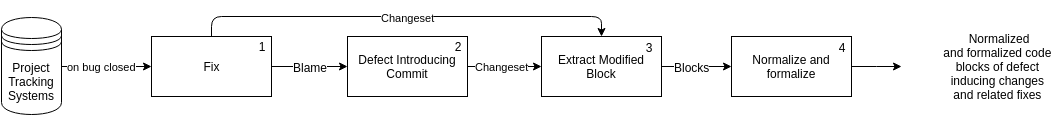
\includegraphics[width=\textwidth]{media/fix-approach.png}
    \caption{Managing events happening on project tracking systems to extract defect-introducing commits and commits that provided the fixes\label{fig:bianca1}}
\end{figure*}

\begin{figure*}
  \centering
    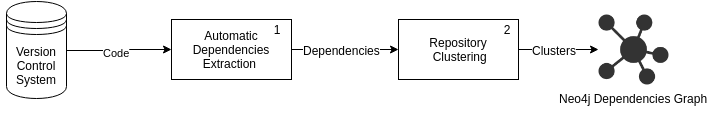
\includegraphics[width=0.7\textwidth]{media/cluster-approach}
    \caption{Clustering by dependency\label{fig:bianca3}}
\end{figure*}

\begin{figure*}
  \centering
    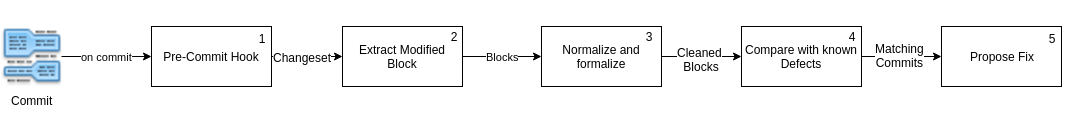
\includegraphics[width=\textwidth]{media/detect-approach}
    \caption{Classifying incoming commits and proposing fixes\label{fig:bianca2}}
\end{figure*}



The project tracking component of BIANCA listens to bug (or issue)
closing events of major open-source projects (currently, BIANCA is
tested with 42 large projects). These projects share many dependencies.
Projects can depend on each other or on common external tools and
libraries. We perform project dependency analysis to identify groups of
highly-coupled projects.

In the second process (Figure \ref{fig:bianca2}), BIANCA identifies
risky commits within each group so as to increase the chances of finding
risky commits caused by project dependencies. For each project group, we
extract code blocks from defect-commits and fix-commits.\\
The extracted code blocks are saved in a database that is used to
identify risky commits before they reach the central repository. For
each match between a risky commit and a defect-commit, we pull out from
the database the corresponding \emph{fix-commit} and present it to the
developer as a potential way to improve the commit content. These phases
are discussed in more detail in the upcoming subsections.

\subsection{Clustering Project Repositories}\label{sec:clustering}

We cluster projects according to their dependencies. The rationale is
that projects that share dependencies are most likely to contain defects
caused by misuse of these dependencies. In this step, the project
dependencies are analysed and saved into a single no-SQL graph database
as shown in Figure \ref{fig:bianca3}. Graph databases use graph
structures as a way to store and query information. In our case, a node
corresponds to a project that is connected to other projects on which it
depends. Project dependencies can be automatically retrieved if projects
use a dependency manager such as Maven.

Figure \ref{fig:network-sample} shows a simplified view of a dependency
graph for a project named \texttt{com.badlogicgames.gdx}. As we can see,
\texttt{badlogicgames.gdx} depends on projects owned by the same
organization (i.e., badlogicgames) and other organizations such as
Google, Apple, and Github.

\begin{figure}
  \centering
    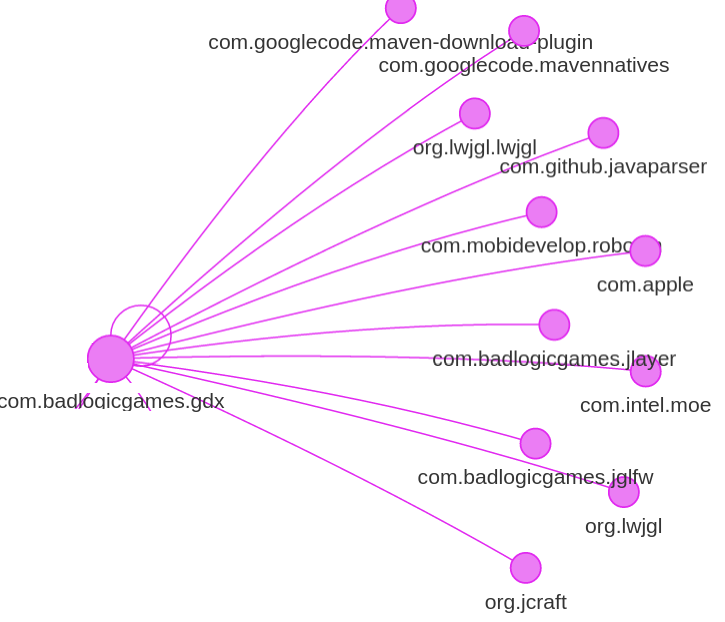
\includegraphics[width=0.40\textwidth]{media/network-sample.png}
    \caption{Simplified Dependency Graph for \texttt{com.badlogicgames.gdx}\label{fig:network-sample}}
\end{figure}

Once the project dependency graph is extracted, we use a clustering
algorithm to partition the graph. To this end, we choose the
Girvan--Newman algorithm {[}@Girvan2002; @Newman2004{]}, used to detect
communities by progressively removing edges from the original network.
The connected components of the remaining network form distinct
communities. Instead of trying to construct a measure that identifies
the edges that are the most central to communities, the Girvan--Newman
algorithm focuses on edges that are most likely ``between'' communities.
This algorithm is very effective at discovering community structure in
both computer-generated and real-world network data {[}@Newman2004{]}.
Other clustering algorithms can also be used.

\subsection{Building a Database of Code Blocks of Defect-Commits and
Fix-Commits}\label{sec:offline}

To build our database of code blocks that are related to defect-commits
and fix-commits, we first need to identify the respective commits. Then,
we extract the relevant blocks of code from the commits.

\textbf{Extracting Commits:} BIANCA listens to bug (or issue) closing
events happening on the project tracking system. Every time an issue is
closed, BIANCA retrieves the commit that was used to fix the issue (the
fix-commit) as well as the one that introduced the defect (the
defect-commit). Retrieving fix-commits, however, is known to be a
challenging task {[}@Wu2011{]}. This is because the link between the
project tracking system and the code version control system is not
always explicit. In an ideal situation, developers would add a reference
to the issue they work on inside the description of the commit. But this
good practice is not always followed. To make the link between
fix-commits and their related issues, we turn to a modified version of
the back-end of commit-guru {[}@Rosen2015a{]}. Commit-guru is a tool,
developed by Rosen \emph{et al.} {[}@Rosen2015a{]} to detect \emph{risky
commits}. In order to identify risky commits, Commit-guru builds a
statistical model using change metrics (i.e., amount of lines added,
amount of lines deleted, amount of files modified, etc.) from past
commits known to have introduced defects in the past.

Commit-guru's back-end has three major components: ingestion, analysis,
and prediction. We reuse the ingestion part of the analysis components
for BIANCA. The ingestion component is responsible for ingesting (i.e.,
downloading) a given repository. Once the repository is entirely
downloaded on a local server, each commit history is analysed. Commits
are classified using the list of keywords proposed by Hindle \emph{et
al.} {[}@Hindle2008{]}. Commit-guru implements the SZZ algorithm
{[}@Kim2006c{]} to detect risky changes, where it performs the SCM
blame/annotate function on all the modified lines of code for their
corresponding files on the fix-commit's parents. This returns the
commits that previously modified these lines of code and are flagged as
the bug introducing commits (i.e., the defect-commits). Priori work
showed that Commit-guru is effective in identifying defect-commits and
their corresponding fixing commits {[}@Kamei2013a{]} and to date, the
SZZ algorithm, which Commit-guru uses, is considered to be the
state-of-the-art in detecting risky commits. Note that we could use a
simpler and more established tool such as Relink {[}@Wu2011{]} to link
the commits to their issues and re-implement the classification proposed
by Hindle \emph{et al.} {[}@Hindle2008{]} on top of it. However,
commit-guru has the advantage of being open-source, making it possible
to modify it to fit our needs and fine-tune its performance.

\textbf{Extracting Code Blocks:} To extract code blocks from fix-commits
and defect-commits, we rely on TXL {[}@Cordy2006a{]}, which is a
first-order functional programming over linear term rewriting, developed
by Cordy et al. {[}@Cordy2006a{]}. For TXL to work, one has to write a
grammar describing the syntax of the source language and the
transformations needed. TXL has three main phases: \emph{parse},
\emph{transform}, \emph{unparse}. In the parse phase, the grammar
controls not only the input but also the output forms. The following
code sample---extracted from the official documentation---shows a
grammar matching an \emph{if-then-else} statement in C with some special
keywords: {[}IN{]} (indent), {[}EX{]} (exdent) and {[}NL{]} (newline)
that will be used in the output form.

\begin{Shaded}
\begin{Highlighting}[]
\KeywordTok{define} \NormalTok{if_statement}
  \KeywordTok{if} \KeywordTok{(} \NormalTok{[}\KeywordTok{expr}\NormalTok{] }\KeywordTok{)} \NormalTok{[}\KeywordTok{IN}\NormalTok{][NL]}
\NormalTok{[}\KeywordTok{statement}\NormalTok{] [EX]}
\NormalTok{[}\KeywordTok{opt} \NormalTok{else_statement]}
\KeywordTok{end} \NormalTok{define}

\KeywordTok{define} \NormalTok{else_statement}
  \KeywordTok{else} \NormalTok{[}\KeywordTok{IN}\NormalTok{][NL]}
\NormalTok{[}\KeywordTok{statement}\NormalTok{] [EX]}
\KeywordTok{end} \NormalTok{define}
\end{Highlighting}
\end{Shaded}

Then, the \emph{transform} phase applies transformation rules that can,
for example, normalize or abstract the source code. Finally, the third
phase of TXL, called \emph{unparse}, unparses the transformed parsed
input to output it. Also, TXL supports what its creators call
\emph{Agile Parsing} {[}@Dean{]}, which allow developers to redefine the
rules of the grammar and, therefore, apply different rules than the
original ones. BIANCA takes advantage of that by redefining the blocks
that should be extracted for the purpose of code comparison, leaving out
the blocks that are out of scope. More precisely, before each commit, we
only extract the blocks belonging to the modified parts of the source
code. Hence, we only process, in an incremental manner, the latest
modification of the source code instead of the source code as a whole.

We have selected TXL for several reasons. First, TXL is easy to install
and to integrate with the normal work flow of a developer. Second, it
was relatively easy to create a grammar that accepts commits as input.
This is because TXL supports C, Java, Csharp, Python and WSDL grammars,
with the ability to customize them to accept changesets (chunks of the
modified source code that include the added, modified, and deleted
lines) instead of the whole code.

\begin{algorithm}
 \KwData{$Changeset[]$ changesets\;
 $Block[]$ prior\_blocks\;
 }
 \KwResult{Up to date blocks of the systems}
 \For{$i \leftarrow 0$ \KwTo$size\_of~changesets$}{
    Block[] blocks $\leftarrow$ $extract\_blocks(changesets)$\;
    \For{$j \leftarrow 0$ \KwTo$size\_of~blocks$}{
       write $blocks[j]$\;
    }
 }

 \SetKwProg{myproc}{Function}{ $~extract\_blocks(Changeset~cs)$}{}
   \myproc{{}}{

   \uIf{$cs~is~unbalanced~right$}{$cs \leftarrow expand\_left(cs)$\;}

   \ElseIf{$cs~is~unbalanced~left$}{$cs \leftarrow expand\_right(cs)$\;}

   \nl\KwRet$txl\_extract\_blocks(cs)$\;
   }


 \caption{Overview of the Extract Blocks Operation\label{alg:extract}}
\end{algorithm}

Algorithm \ref{alg:extract} presents an overview of the \emph{extract}
and \emph{save} blocks operations of BIANCA. This algorithm receives as
argument, the changesets and the blocks that have been previously
extracted. Then, Lines 1 to 5 show the \(for\) loop that iterates over
the changesets. For each changeset (Line 2), we extract the blocks by
calling the \(~extract\_blocks(Changeset~cs)\) function. In this
function, we expand our changeset to the left and to the right in order
to have a complete block.

As depicted below, changesets contain only the modified chunk of code
and not necessarily complete blocks.

\begin{Shaded}
\begin{Highlighting}[]
\DataTypeTok{@@ -315,36 +315,6 @@}
\NormalTok{int initprocesstree_sysdep}
\NormalTok{(ProcessTree_T **reference) \{}
    \NormalTok{mach_port_deallocate(mytask,}
      \NormalTok{task);}
\NormalTok{\}}
\NormalTok{\}}
\StringTok{- if (task_for_pid(mytask, pt[i].pid,}
\StringTok{-  &task) == KERN_SUCCESS) \{}
\StringTok{-   mach_msg_type_number_t   count;}
\StringTok{-   task_basic_info_data_t   taskinfo;}
\end{Highlighting}
\end{Shaded}

Therefore, we need to expand the changeset to the left (or right) to
have syntactically correct blocks. We do so by checking the block's
beginning and ending with a parentheses algorithms
{[}@bultena1998eades{]}. Then, we send these expanded changesets to TXL
for block extraction and formalization.

One important note about this database is that the process can be
cold-started. A tool supporting BIANCA does not need to \emph{wait} for
a project to have issues and fixes to be in effect. It can leverage the
defect-commits and fix-commits of projects in the same cluster that
already have a history. Therefore, BIANCA is applicable at the beginning
of every project. The only requirement is to use a dependency manager.

\subsection{Analysing New Commits Using Pre-Commit
Hooks}\label{sec:online}

Each time a developer makes a commit, BIANCA intercepts it using a
pre-commit hook, extracts the corresponding code block (in a similar way
as in the previous phase), and compares it to the code blocks of
historical defect-commits. If there is a match then the new commit is
deemed to be risky. A threshold \(\alpha\) is used to assess the extent
beyond which two commits are considered similar. The setting of
\(\alpha\) is discussed in the case study section.

Pre-commit hooks are custom scripts set to fire off when certain
important actions of the versionning process occur. There are two groups
of hooks: client-side and server-side. Client-side hooks are triggered
by operations such as committing and merging, whereas server-side hooks
run on network operations such as receiving pushed commits. These hooks
can be used for all sorts of reasons such as checking compliance with
coding rules or automatic run of unit test suites. The pre-commit hook
runs before the developer specifies a commit message. It is used to
inspect the modifications that are about to be committed. BIANCA is
based on a set of bash and python scripts, and the entry point of these
scripts lies in a pre-commit hook. These scripts intercept the commit
and extract the corresponding code blocks.

To compare the extracted blocks to the ones in the database, we resort
to clone detection techniques, more specifically, text-based clone
detection techniques. This is because lexical and syntactic analysis
approaches (alternatives to text-based comparisons) would require a
complete program to work, i.e., a program that compiles. In the
relatively wide-range of tools and techniques that exist to detect
clones by considering code as text {[}@Johnson1993; @Johnson1994;
@Marcus; @Manber1994; @StephaneDucasse; @Wettel2005{]}, we selected
NICAD as the main text-based method for comparing code blocks
{[}@Cordy2011{]} for several reasons. First, NICAD is built on top of
TXL, which we also used in the previous phase. Second, NICAD can detect
Types 1, 2 and 3 software clones {[}@CoryKapser{]}. Type 1 clones are
copy-pasted blocks of code that only differ from each other in terms of
non-code artefacts such as indentation, whitespaces, comments and so on.
Type 2 clones are blocks of code that are syntactically identical except
literals, identifiers, and types that can be modified. Also, Type 2
clones share the particularities of Type 1 about indentation,
whitespaces, and comments. Type 3 clones are similar to Type 2 clones in
terms of modification of literals, identifiers, types, indentation,
whitespaces, and comments but also contain added or deleted code
statements. BIANCA detects Type 3 clones since they can contain added or
deleted code statements, which make them suitable for comparing commit
code blocks.

NICAD works in three phases: \emph{Extraction}, \emph{Comparison} and
\emph{Reporting}. During the \emph{Extraction} phase all potential
clones are identified, pretty-printed, and extracted. We do not use the
\emph{Extraction} phase of NICAD as it has been built to work on
programs that are syntactically correct, which is not the case for
changesets. We replaced NICAD's \emph{Extraction} phase with our scripts
for building code blocks (described in the previous phase).

In the \emph{Comparison} phase, the extracted blocks are transformed,
clustered and compared to find potential clones. Using TXL sub-programs,
blocks go through a process called pretty-printing where they are
stripped of formatting and comments. When code fragments are cloned,
some comments, indentation or spacing are changed according to the new
context where the new code is used. This pretty-printing process ensures
that all code will have the same spacing and formatting, which renders
the comparison of code fragments easier. Furthermore, in the
pretty-printing process, statements can be broken down into several
lines. Table \ref{tab:pretty-printing} {[}@Iss2009{]} shows how this can
improve the accuracy of clone detection with three \texttt{for}
statements, \texttt{for\ (i=0;\ i\textless{}10;\ i++)},
\texttt{for\ (i=1;\ i\textless{}10;\ i++)} and
\texttt{for\ (j=2;\ j\textless{}100;\ j++)}. The pretty-printing allows
NICAD to detect Segments 1 and 2 as a clone pair because only the
initialization of \(i\) changed. This specific example would not have
been marked as a clone by other tools we tested such as Duploc
{[}@Ducasse1999{]}. In addition to the pretty-printing, code can be
normalized and filtered to detect different classes of clones and match
user preferences.

\begin{table}[]
\centering
\caption{Pretty-Printing Example}
\label{tab:pretty-printing}
\resizebox{0.5\textwidth}{!}{%
\begin{tabular}{l|l|l|l|l|l}
\hline
Segment 1          & Segment 2          & Segment 3           & S1 \& S2 & S1 \& S3 & S2 \& S3 \\ \hline \hline
for (              & for (              & for (               & 1        & 1        & 1        \\
i = 0;             & i = 1;             & j = 2;              & 0        & 0        & 0        \\
i \textgreater 10; & i \textgreater 10; & j \textgreater 100; & 1        & 0        & 0        \\ 
i++)               & i++)               & j++)                & 1        & 0        & 0        \\ \hline \hline
\multicolumn{3}{c|}{Total Matches}                            & 3        & 1        & 1        \\ \hline
\multicolumn{3}{c|}{Total Mismatches}                         & 1        & 3        & 3 \\ \hline

\end{tabular}
}
\end{table}


The extracted, pretty-printed, normalized and filtered blocks are marked
as potential clones using a Longest Common Subsequence (LCS) algorithm
{[}@Hunt1977{]}. Then, a percentage of unique statements can be computed
and, given the threshold \(\alpha\), the blocks are marked as clones.

Another important aspect of the design of BIANCA is the ability to
provide guidance to developers on how to improve the risky commits. We
achieve this by extracting from the database the fix-commit
corresponding to the matching defect-commit and present it to the
developer. We believe that this makes BIANCA a practical approach for
the developers as they will know why a given modification has been
reported as risky in terms of code; this is something that is not
supported by techniques based on statistical models (e.g.,
{[}@Kamei2013a; @Rosen2015a{]}).\\
A tool that supports BIANCA should have enough flexibility to allow
developers to enable or disable the recommendations made by BIANCA.
Furthermore, because BIANCA acts before the commit reaches the central
repository, it prevents unfortunate pulls of defects by other members of
the organization.

\section{Case Study Setup}\label{sec:exp}

In this section, we present the setup of our case study in terms of
repository selection, dependency analysis, comparison process and
evaluation measures.

\subsection{Project Repository Selection}\label{sec:rep}

To select the projects used to evaluate our approach, we followed three
simple criteria. First, the projects need to be in Java and use Maven to
manage dependencies. This way, we can automatically extract the
dependencies and perform the clustering of projects. The second
criterion is to have projects that enjoy a large community support and
interest. We selected projects that have at least 2000 followers. A
different threshold could be used. Finally, the projects must have a
public issue repository to be able to mine their past issues and the
fixes. We queried Github with these criteria and retrieved 42 projects
(see Table \ref{tab:results} for the list of projects), including those
from some of major open-source contributors such as Alibaba, Apache
Software Foundation, Eclipse, Facebook, Google and Square.

\subsection{Project Dependency Analysis}\label{sec:dependencies}

Figure \ref{fig:dep-graph} shows the project dependency graph. The
dependency graph is composed of 592 nodes divided into five clusters
shown in yellow, red, green, purple and blue. The size of the nodes in
Figure \ref{fig:dep-graph} is proportional to the number of connections
from and to the other nodes.

\begin{figure}
  \centering
    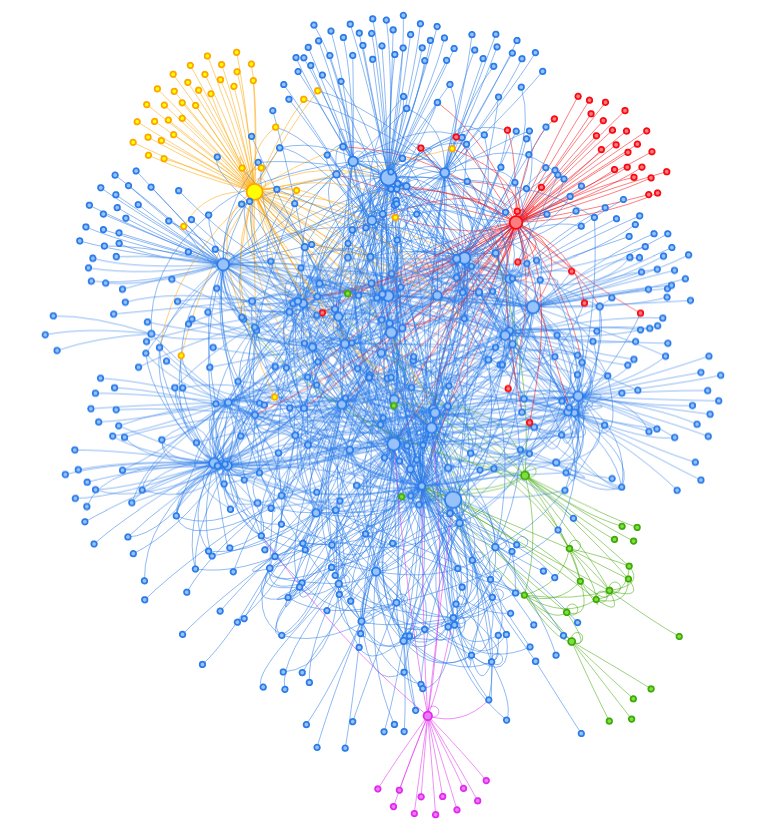
\includegraphics[width=0.35\textwidth]{media/network.png}
    \caption{Dependency Graph\label{fig:dep-graph}}
\end{figure}

As shown in Figure \ref{fig:dep-graph}, these Github projects are very
much interconnected.\\
In average, the projects composing our dataset have 77 dependencies.
Among the 77 dependencies, in average, 62 dependencies are shared with
at least one other project from our dataset.

Table \ref{tab:communities} shows the result of the Girvan--Newman
clustering algorithm in terms of centroids and betweenness. The blue
cluster is dominated by Storm from The Apache Software Foundation. Storm
is a distributed real-time computation system. Druid by Alibaba, the
e-commerce company that provides consumer-to-consumer,
business-to-consumer and business-to-business sales services via web
portals, dominates the yellow cluster. In recent years, Alibaba has
become an active member of the open-source community by making some of
its projects publicly available. The red cluster has Hadoop by the
Apache Software Foundation as its centroid. Hadoop is an open-source
software framework for distributed storage and distributed processing of
very large data sets on computer clusters built from commodity hardware.
The green cluster is dominated by the Persistence project of OpenHab.
OpenHab proposes home automation solutions and the Persistence project
is their data access layer. Finally, the purple cluster is dominated by
Libdx by Badlogicgames, which is a cross-platform framework for game
development.

A review of each cluster shows that this partitioning divides projects
in terms of high-level functionalities. For example, the blue cluster is
almost entirely composed of projects from the Apache Software
Foundation. Projects from the Apache Software Foundation tend to build
on top of one another. We also have the red cluster for Hadoop, which is
by itself an ecosystem inside the Apache Software Foundation. Finally,
we obtained a cluster for e-commerce applications (yellow), real-time
network application for home automation (green), and game development
(purple).


\begin{table}[]
\centering
\caption{Communities in terms of ID, Color code, Centroids, Betweenness and number of members}
\label{tab:communities}
\begin{tabular}{llllcc}
\hline
\#ID               & Community             & Centroids        & Betweenness & \# Members        \\ \hline
1                  & Blue                  & Storm &           24,525 &    479                                      \\ \hline
2                  & Yellow                & Alibaba          & 24,400      & 42                                      \\ \hline
3                  & Red                   & Hadoop           & 16,709      & 37                                      \\ \hline
4                  & Green                 & Openhab          & 3,504       & 22                                      \\ \hline
5                  & Purple                & Libdx              & 6,839       & 12  \\ \hline                                
\end{tabular}
\end{table}


\subsection{Building a Database of Defect-Commits and Fix-Commits for
Performances Evaluation}\label{sub:golden}

To build the database against which we assess the performance of BIANCA,
we use the same process as discussed in Section \ref{sec:offline}. We
used Commit-guru to retrieve the complete history of each project and
label commits as defect-commits if they appear to be linked to a closed
issue. The process used by Commit-guru to identify commits that
introduce a defect is simple and reliable in terms of accuracy and
computation time {[}@Kamei2013{]}. We use the commit-guru labels as the
baseline to compute the precision and recall of BIANCA. Each time BIANCA
classifies a commit as \emph{risky}, we can check if the \emph{risky}
commit is in the database of defect-introducing commits. The same
evaluation process is used by related studies {[}@ElEmam2001; @Lee2011a;
@Bhattacharya2011; @Kpodjedo2010{]}. The difference between this
\emph{golden} database and the database described in Section
\ref{sec:offline} is that, with this one, we unwind the whole history
instead of building the history as it happens.

\subsection{Process of Comparing New Commits}\label{sec:newcommits}

Because our approach relies on commit pre-hooks to detect risky commit,
we had to find a way to \emph{replay} past commits. To do so, we
\emph{cloned} our test subjects, and then created a new branch called
\emph{BIANCA}. When created, this branch is reinitialized at the initial
state of the project (the first commit) and each commit can be replayed
as they have originally been. For each commit, we store the time taken
for \emph{BIANCA} to run, the number of detected clone pairs, and the
commits that match the current commit. As an example, let's assume that
we have three commits from two projects. At time \(t_1\), commit \(c_1\)
in project \(p_1\) introduces a defect. The defect is experienced by an
user that reports it via an issue \(i_1\) at \(t_2\). A developer fixes
the defect introduced by \(c_1\) in commit \(c_2\) and closes \(i_1\) at
\(t_3\). From \(t_3\) we known that \(c_1\) introduced a defect using
the process described in Section \ref{sub:golden}. If at \(t_4\),
\(c_3\) is pushed to \(p_2\) and \(c_3\) matches \(c_1\) after
preprocessing, pretty-printing and formatting, then \(c_3\) is
classified as \emph{risky} by BIANCA and \(c_2\) is proposed to the
developer as a potential solution for the defect introduced in \(c_3\).

\begin{figure}

\begin{tikzpicture}
\begin{axis}[
xlabel={Similarity Threshold $\alpha$},
ylabel={Precentage},
legend pos=north west,
xmin=0,
xmax=100
]
\addplot +[mark=none] table [x=alpha, y=f1, col sep=comma] {data/alpha.csv};
\addlegendentry{F$_1$-measure}
\addplot +[mark=none] table [x=alpha, y=precision, col sep=comma] {data/alpha.csv};
\addlegendentry{Precision}
\addplot +[mark=none] table [x=alpha, y=recall, col sep=comma] {data/alpha.csv};
\addlegendentry{Recall}
\node[label={360:{$\alpha$=35\%}},circle,fill,inner sep=2pt] at (axis cs:35,45.6890364256) {};
\end{axis}
\end{tikzpicture}
\caption{Precision, Recall and F$_1$-measure variations according to $\alpha$\label{fig:alpha-deter}}
\end{figure}

To measure the similarity between pairs of commits, we need to decide on
the value of \(\alpha\). One possibility would be to test for all
possible values of \(\alpha\) and pick the one that provides best
accuracy (F\(_1\)-measure). The ROC (Receiver Operating Characteristic)
curve can then be used to display the performance of BIANCA with
different values of \(\alpha\). Running experiments with all possible
\(\alpha\) turned out to be computationally demanding given the large
number of commits. Testing with all the different values of \(\alpha\)
amounts to 4e10 comparisons.

To address this, we randomly selected a sample of 1\% commits from our
dataset and checked the results by varying \(\alpha\) from 1 to 100\%.
Figure \ref{fig:alpha-deter} shows the results. As we can see, there is
a tradeoff between precision and recall, however, after the \(\alpha\) =
35\% point, we see a drop in recall; hence, we set \(\alpha\) = 35\% in
our experiments. It should also be noted that in clone detection work a
threshold of around 30\% is considered an adequate threshold above which
two code blocks are deemed to be clones, especially for clones of Type
3, which contain added or deleted code statements {[}@Roy2008;
@Cordy2011{]}. With \(\alpha\) = 35\%, the experiments took nearly three
months to run on 48 Amazon VPS (Virtual Private Server) running in
parallel (4e8 comparisons).

\subsection{Evaluation Measures}\label{evaluation-measures}

Similar to prior work focusing on risky commits (e.g.,
{[}@SunghunKim2008; @Kamei2013{]}), we used precision, recall, and
F\(_1\)-measure to evaluate our approach. They are computed using TP
(true positives), FP (false positives), FN (false negatives), which are
defined as follows:

\begin{itemize}
\tightlist
\item
  TP: is the number of defect-commits that were properly classified by
  BIANCA
\item
  FP: is the number of healthy commits that were classified by BIANCA as
  risky
\item
  FN: is the number of defect introducing-commits that were not detected
  by BIANCA
\item
  Precision: TP / (TP + FP)
\item
  Recall: TP / (TP + FN)
\item
  F\(_1\)-measure: 2.(precision.recall)/(precision+recall)
\end{itemize}

It is worth mentioning that, in the case of defect prevention, false
positives can be hard to identify as the defects could be in the code
but not yet reported through a bug report (or issue). To address this,
we did not include the last six months of history. Following similar
studies {[}@Rosen2015; @Chen2014; @Rosen2015a; @Shihab2013{]}, if a
defect is not reported within six months then it is not considered.

\section{Case Study Results}\label{sec:result}

In this section, we show the effectiveness of BIANCA in detecting risky
commits using clone detection and project dependency analysis. The main
research question addressed by this case study is: Can we detect risky
commits using code comparison within and across related projects, and if
so, what would be the accuracy?

% Please add the following required packages to your document preamble:
% \usepackage{multirow}
% \usepackage{graphicx}
% \usepackage[normalem]{ulem}
% \useunder{\uline}{\ul}{}
\begin{table*}[]
\centering
\caption{BIANCA results in terms of organization, project name, a short description, number of class, number of commits, number of defect introducing commits, number of risky commit detected, precision (\%), recall (\%), F$_1$-measure (\%), the average similarity of first 3 and 5 proposed fixes with the actual fix and the average time difference between detected and original.}
  \label{tab:results}
\resizebox{\textwidth}{!}{%
\begin{tabular}{lllccccccccc}
\hline
Organization                & Project Name                                                  & Short Description                                                        & NoC             & \#Commits        & \begin{tabular}[c]{@{}c@{}}Bug  \\Introducing\\ Commit\end{tabular} & Detected       & Precision      & Recall         & F$_1$          & \begin{tabular}[c]{@{}c@{}}Top 3 \\ Fixes \\Similarity\end{tabular} & \begin{tabular}[c]{@{}c@{}}Top 5\\ Fixes\\ Similarity\end{tabular} \\ \hline
\multirow{4}{*}{Alibaba}    & druid                                                         & Database connection pool                                                 & 3,309           & 4,775            & 1,260                                                            & 787            & 88.44          & 62.46          & 73.21          & 39.97                                                             & 46.69                                                              \\
                            & dubbo                                                         & RPC framework                                                            & 1,715           & 1,836            & 119                                                              & 61             & 96.72          & 51.26          & 67.01          & 60.01                                                             & 57.14                                                              \\
                            & fastjson                                                      & JSON parser/generator                                                    & 2,002           & 1,749            & 516                                                              & 373            & 95.71          & 72.29          & 82.37          & 18.19                                                             & 15.23                                                              \\
                            & jstorm                                                        & Stream Process                                                           & 1,492           & 215              & 24                                                               & 21             & 90.48          & 87.50          & 88.96          & 22.38                                                             & 30.48                                                              \\ \hline
\multirow{2}{*}{Apache}     & hadoop                                                        & Distributed processing                                                   & 9,108           & 14,154           & 3,678                                                            & 851            & 86.84          & 23.14          & 36.54          & 38.94                                                             & 47.68                                                              \\
                            & storm                                                         & Realtime system                                                          & 2,209           & 7,208            & 951                                                              & 444            & 86.26          & 46.69          & 60.58          & 53.03                                                             & 61.10                                                              \\ \hline
Clojure                     & clojure                                                       & Programming language                                                     & 335             & 2,996            & 596                                                              & 46             & 86.96          & 7.72           & 14.18          & 53.61                                                             & 59.52                                                              \\ \hline
\multirow{2}{*}{Dropwizard} & dropwizard                                                    & RESTful web services                                                     & 964             & 3,809            & 581                                                              & 179            & 96.65          & 30.81          & 46.72          & 47.54                                                             & 53.56                                                              \\
                            & metrics                                                       & JVM metrics                                                              & 335             & 1,948            & 331                                                              & 129            & 95.35          & 38.97          & 55.33          & 22.53                                                             & 31.82                                                              \\ \hline
Eclipse                     & che                                                           & Eclipse IDE                                                              & 7,818           & 1,826            & 169                                                              & 9              & 88.89          & 5.33           & 10.05          & 31.01                                                             & 39.04                                                              \\ \hline
Excilys                     & \begin{tabular}[c]{@{}l@{}}Android\\ Annotations\end{tabular} & Android Development                                                      & 1,059           & 2,582            & 566                                                              & 9              & 100.00         & 1.59           & 3.13           & 25.60                                                             & 32.13                                                              \\ \hline
Facebook                    & fresco                                                        & Images Management                                                        & 1,007           & 744              & 100                                                              & 68             & 92.65          & 68.00          & 78.43          & 64.14                                                             & 71.03                                                              \\ \hline
Gocd                        & gocd                                                          & Continuous Delivery server                                               & 16,735          & 3,875            & 499                                                              & 297            & 91.58          & 59.52          & 72.15          & 21.62                                                             & 30.59                                                              \\ \hline
\multirow{4}{*}{Google}     & auto                                                          & source code generators                                                   & 257             & 668              & 124                                                              & 95             & 100.00         & 76.61          & 86.76          & 47.66                                                             & 55.70                                                              \\
                            & guava                                                         & Google Libraries for Java 6+                                             & 1,731           & 3,581            & 973                                                              & 592            & 98.48          & 60.84          & 75.22          & 23.74                                                             & 23.59                                                              \\
                            & guice                                                         & Dependency injection                                                     & 716             & 1,514            & 605                                                              & 104            & 85.58          & 17.19          & 28.63          & 34.77                                                             & 34.53                                                              \\
                            & iosched                                                       & Android App                                                              & 1,088           & 129              & 9                                                                & 6              & 100.00         & 66.67          & 80.00          & 16.50                                                             & 24.97                                                              \\ \hline
Gradle                      & gradle                                                        & Build system                                                             & 11,876          & 37,207           & 6,896                                                            & 1,557          & 97.50          & 22.58          & 36.67          & 23.58                                                             & 19.93                                                              \\ \hline
Jankotek                    & mapdb                                                         & Concurrent datastructures                                                & 267             & 1,913            & 691                                                              & 440            & 94.32          & 63.68          & 76.03          & 63.16                                                             & 72.48                                                              \\ \hline
Jhy                         & jsoup                                                         & Parser                                                                   & 136             & 917              & 254                                                              & 153            & 87.58          & 60.24          & 71.38          & 46.41                                                             & 44.59                                                              \\ \hline
Libdx                       & libgdx                                                        & Java game development                                                    & 4,679           & 12,497           & 3,514                                                            & 1,366          & 87.70          & 38.87          & 53.87          & 57.70                                                             & 56.31                                                              \\ \hline
Netty                       & netty                                                         & Event-driven application                                                 & 2,383           & 7,580            & 3,991                                                            & 1,618          & 89.43          & 40.54          & 55.79          & 63.41                                                             & 62.67                                                              \\ \hline
Openhab                     & openhab                                                       & Home Automation Bus                                                      & 5,817           & 8,826            & 28                                                               & 2              & 100.00         & 7.14           & 13.33          & 28.46                                                             & 30.66                                                              \\ \hline
Openzipkin                  & zipkin                                                        & Distributed tracing system                                               & 397             & 799              & 176                                                              & 73             & 87.67          & 41.48          & 56.31          & 55.92                                                             & 51.90                                                              \\ \hline
Orfjackal                   & retrolambda                                                   & Backport of Java 8's lambda                                              & 171             & 447              & 97                                                               & 35             & 94.29          & 36.08          & 52.19          & 34.69                                                             & 42.06                                                              \\ \hline
OrientTechnologie           & orientdb                                                      & Multi-Model DBMS                                                         & 2,907           & 13,907           & 7,441                                                            & 2,894          & 86.77          & 38.89          & 53.71          & 62.20                                                             & 70.00                                                              \\ \hline
Perwendel                   & spark                                                         & Sinatra  for java                                                        & 205             & 703              & 125                                                              & 82             & 97.56          & 65.60          & 78.45          & 21.88                                                             & 28.00                                                              \\ \hline
PrestoDb                    & presto                                                        & Distributed SQL query                                                    & 4,381           & 8,065            & 2,112                                                            & 991            & 90.62          & 46.92          & 61.83          & 23.34                                                             & 20.64                                                              \\ \hline
RoboGuice                   & roboguice                                                     & Google Guice on Android                                                  & 1,193           & 1,053            & 229                                                              & 70             & 91.43          & 30.57          & 45.82          & 53.81                                                             & 56.55                                                              \\ \hline
Lombok                      & lombok                                                        & \begin{tabular}[c]{@{}l@{}}Additions to the\\ Java language\end{tabular} & 1,146           & 1,872            & 560                                                              & 212            & 91.98          & 37.86          & 53.64          & 58.94                                                             & 57.49                                                              \\ \hline
Scribejava                  & scribejava                                                    & OAuth library                                                            & 218             & 609              & 72                                                               & 16             & 93.75          & 22.22          & 35.93          & 30.05                                                             & 38.16                                                              \\ \hline
\multirow{6}{*}{Square}     & dagger                                                        & Dependency injector                                                      & 232             & 697              & 144                                                              & 84             & 90.48          & 58.33          & 70.93          & 64.29                                                             & 64.97                                                              \\
                            & javapoet                                                      & Java API                                                                 & 66              & 650              & 163                                                              & 113            & 100.00         & 69.33          & 81.88          & 51.04                                                             & 53.20                                                              \\
                            & okhttp                                                        & HTTP+HTTP/2 client                                                       & 344             & 2,649            & 592                                                              & 474            & 93.04          & 80.07          & 86.07          & 29.09                                                             & 24.91                                                              \\
                            & okio                                                          & I/O API for Java                                                         & 90              & 433              & 40                                                               & 24             & 100.00         & 60.00          & 75.00          & 31.51                                                             & 35.50                                                              \\
                            & otto                                                          & Guava-based event bus                                                    & 84              & 201              & 15                                                               & 15             & 93.33          & 100.00         & 96.55          & 54.11                                                             & 49.94                                                              \\
                            & retrofit                                                      & Type-safe HTTP client                                                    & 202             & 1,349            & 151                                                              & 111            & 99.10          & 73.51          & 84.41          & 49.88                                                             & 45.46                                                              \\ \hline
StephaneNicolas             & robospice                                                     & Android library                                                          & 461             & 865              & 113                                                              & 39             & 87.18          & 34.51          & 49.45          & 60.90                                                             & 65.04                                                              \\ \hline
ThinkAurelius               & titan                                                         & Graph Database                                                           & 2,015           & 4,434             & 1,634                                                            & 527            & 90.13          & 32.25          & 47.51          & 48.64                                                             & 50.59                                                              \\ \hline
Jedis                       & jedis                                                         & Redis client                                                             & 203             & 1,370             & 295                                                              & 226            & 92.04          & 76.61          & 83.62          & 25.69                                                             & 29.45                                                              \\ \hline
Yahoo                       & anthelion                                                     & Plugin for Apache Nutch                                                  & 1,620            & 7                & 0                                                                & -              & -              & -              & -              & -                                                                 & -                                                                  \\ \hline
Zxing                       & zxing                                                         & 1D/2D barcode image                                                      & 3,030           & 3,253            & 791                                                              & 123            & 94.31          & 15.55          & 26.70          & 29.35                                                             & 37.96                                                              \\ \hline
\textbf{Total}              & \textbf{}                                                     & \textbf{}                                                                & \textbf{96,003} & \textbf{165,912} & \textbf{41,225}                                                  & \textbf{15316} & \textbf{90.75} & \textbf{37.15} & \textbf{52.72} & \textbf{40.78}                                                    & \textbf{44.17}                                                     \\ \hline
\end{tabular}%
}
\end{table*}

Table \ref{tab:results} shows the results of applying BIANCA in terms of
the organization, project name, a short description of the project, the
number of classes, the number of commits, the number of defect-commits,
the number of defect-commits detected by BIANCA, precision (\%), recall
(\%), F\(_1\)-measure and the average difference, in days, between
detected commit and the \emph{original} commit inserting the defect for
the first time.

With \(\alpha\) = 35\%, BIANCA achieves, on average, a precision of
90.75\% (13,899/15,316) commits identified as risky. These commits
triggered the opening of an issue and had to be fixed later on. On the
other hand, BIANCA achieves, on average, 37.15\% recall (15,316/41,225),
and an average F\(_1\) measure of 52.72\%. The relatively \emph{low}
recall is to be expected, since BIANCA considers risky commits that are
also in other projects.

Also, out of the 15,316 commits BIANCA classified as \emph{risky}, only
1,320 (8.6\%) were because they were matching a defect-commit inside the
same project. This finding supports the idea that developers of a
project are not likely to introduce the same defect twice while
developers of different projects that share dependencies are, in fact,
likely to introduce similar defects. We believe this is an important
finding for researchers aiming to achieve cross-project defect
prevention, regardless of the technique (e.g., statistical model, AST
comparison, code comparison, etc.) employed.

It is important to note that we do not claim that 37.15\% of issues in
open-source systems are caused by project dependencies. To support such
a claim, we would need to analyse the 15,316 detected defect-commits and
determine how many yield defects that are similar across projects.
Studying the similarity of defects across projects is a complex task and
may require analysing the defect reports manually. This is left as
future work. This said, we showed, in this paper, that software systems
sharing dependencies also share common issues, irrespective to whether
these issues represent similar defects or not.

In the following subsections, we compare BIANCA with a random
classifier, assess the quality of the proposed fixes, and present the
findings of our manual analysis.

\subsection{Random Classifier
Comparison}\label{random-classifier-comparison}

Although our average F\(_1\) measure of 52.72\% may seem low at first
glance, achieveing a high F\(_1\) measure for unbalanced data is very
difficult {[}@menzies2007problems{]}. Therefore, a common appraoch to
ground detection results is to compare it to a simple baseline.

The random classifier first generates a random number \(n\) between 0
and 1 for the 165,912 commits composing our dataset. For each commit, if
\(n\) is greater than 0.5, then the commit is classified as risky and
vice versa. As expected by a random classifier, our implementation
detected \textasciitilde{}50\% (82,384 commits) of the commits to be
\emph{risky}. It is worth mentioning is that the random classifier
achieved 24.9\% precision, 49.96\% recall and 33.24\% F\(_1\)-measure.
Since our data is unbalanced (i.e., there are many more \emph{healthy}
than \emph{risky} commits) these numbers are to be expected for a random
classifier. Indeed, the recall is very close to 50\% since a commit can
take on one of two classifications, risky or non-risky. While analysing
the precision, however, we can see that the data is unbalanced (a random
classifier would achieve a precision of 50\% on a balanced dataset).

It is important to note that the purpose of this analysis is not to say
that we outperform a simple random classifier, rather to shed light on
the fact that our dataset is unbalanced and achieving an average F\(_1\)
= 52.72\% is non-trivial, especially when a baseline only achieves an
F\(_1\)-measure of 33.24\%.

\subsection{Analysis of the Quality of the Fixes Proposed by
BIANCA}\label{analysis-of-the-quality-of-the-fixes-proposed-by-bianca}

One of the advantages of BIANCA over other techniques is that it also
proposes fixes for the \emph{risky} commits it detects. In order to
evaluate the quality of the proposed fixes, we compare the proposed
fixes with the actual fixes provided by the developers. To do so, we
used the same preprocessing steps we applied to incoming commits:
extract, pretty-print, normalize and filter the blocks modified by the
proposed and actual fixes. Then, the blocks of the actual fixes and the
proposed fixes can be compared with our clone comparison engine.

Similar to other studies recommending fixes, we assess the quality of
the first 3 and 5 proposed fixes {[}@Pan2008; @Kim2013;
@tao2014automatically; @Dallmeier; @le2012systematic; @le2015should{]}.
The average similarity of the first 3 fixes is 40.78\% while the
similarity of the first five fixes is 44.17\%. Results are reported in
Table \ref{tab:results}.

In the framework of this study, for a fix to be ranked as qualitative it
has to reach our \(\alpha\)=35\% similarity threshold. Meaning that the
proposed fixed must be at least 35\% similar to the actual fix. On
average, the proposed fixes are above the \(\alpha\)=35\% threshold. On
a per commit basis, BIANCA proposed 101,462 fixes for the 13,899 true
positives \emph{risky commits} (7.3 per commit). Out of the 101,462
proposed fixes, 78.67\% are above our \(\alpha\)=35\% threshold.

In other words, BIANCA is able to detect \emph{risky} commits with
90.75\% precision, 37.15\% recall, and proposes fixes that contain, on
average, 40-44\% of the actual code needed to transform the \emph{risky}
commit into a \emph{non-risky} one. It is still too early to claim
whether BIANCA's recommendations can be useful to developers. For this,
we need to conduct user study, which we plan to do as future work.

\subsection{Manual Analysis}\label{manual-analysis}

BIANCA performed best when applied to three projects: Otto by Square
(100.00\% precision and 76.61\% recall, 96.55\% F\(_1\)-measure), JStorm
by Alibaba (90.48\% precision, 87.50\% recall, 88.96\% F\(_1\)-measure),
and Auto by Google (90.48\% precision, 87.50\% recall, 86.76\%
F\(_1\)-measure). It performed worst when applied to Android Annotations
by Excilys (100.00\% precision, 1.59\% recall, 3.13\% F\(_1\)-measure)
and Che by Eclipse (88.89\% precision, 5.33\% recall, 10.05\%
F\(_1\)-measure), Openhab by Openhab (100.00\% precision, 7.14\% recall,
13.33\% F\(_1\)-measure). To understand the performance of BIANCA, we
conducted a manual analysis of the commits classified as \emph{risky} by
BIANCA for these projects.

\subsubsection{\texorpdfstring{Otto by Square (F\(_1\)-measure =
96.5\%)}{Otto by Square (F\_1-measure = 96.5\%)}}\label{otto-by-square-f_1-measure-96.5}

At first, the F\(_1\)-measure of Otto by Square seems surprising given
the specific set of features it provides. Otto provides a Guava-based
event bus. While it does have dependencies that makes it vulnerable to
defects in related projects, the fact that it provides specific features
makes it, at first sight, unlikely to share defects with other projects.
Through our manual analysis, we found that out of the 16 \emph{risky}
commits detected by BIANCA, only 11 (68.75\%) matched defect-introducing
commits inside the Otto project itself. This is significantly higher
than the average number of single-project defects (8.6\%). Further
investigation of the project management system revealed that a very few
issues have been submitted for this project (15) and, out of the 11
matches inside the Otto project, 7 were aiming to fix the same issue
that had been submitted and fixed several times instead of re-opening
the original issue.

\subsubsection{\texorpdfstring{JStorm by Alibaba (F\(_1\)-measure =
88.96\%)}{JStorm by Alibaba (F\_1-measure = 88.96\%)}}\label{jstorm-by-alibaba-f_1-measure-88.96}

For JStorm by Alibaba, our manual analysis of the \emph{risky} commits
revealed that, in addition to providing stream processes, JStorm mainly
supports JSON. The commits detected as \emph{risky} were related to the
JSON encoding/decoding functionalities of JStorm. In our dataset, we
have several other projects that supports JSON encoding and decoding
such as FastJSON by Alibaba, Hadoop by Apache, Dropwizard by Dropwizard,
Gradle by Gradle and Anthelion by Yahoo. There is, however, only one
project supporting JSON in the same cluster as JStorm, Fastjson by
Alibaba. FastJSON has a rather large history of defect-commits (516) and
18 out of the 21 commits marked as \emph{risky} by BIANCA were marked so
because they matched defect-commits in the FastJSON project.

\subsubsection{\texorpdfstring{Auto by Google (F\(_1\)-measure =
86.76\%)}{Auto by Google (F\_1-measure = 86.76\%)}}\label{auto-by-google-f_1-measure-86.76}

Google Auto is a code generation engine. This code generation engine is
used by other Google projects in our database, such as Guava and Guice.
Most of the Google Auto \emph{risky} commits (79\%) matched commits in
the Guava and the Guice project. As Guice and Guave share the same
code-generation engine (Auto), it makes sense that code introducing
defects in these projects share the characteristics of commits
introducing defects in Auto.

\subsubsection{\texorpdfstring{Openhab by Openhab (F\(_1\)-measure =
13.33\%)}{Openhab by Openhab (F\_1-measure = 13.33\%)}}\label{openhab-by-openhab-f_1-measure-13.33}

Openhab by Openhab provides bus for home automation or smart homes. This
is a very specific set of feature. Moreover, Openhab and its
dependencies are alone in the green cluster. In other words, the only
project against which BIANCA could have checked for matching defects is
Openhab itself. BIANCA was able to detect 2/28 bugs for Openhab. We
believe that if we had other home-automation projects in our dataset
(such as \emph{HomeAutomation} a component based for smart home systems
{[}@Seinturier2012{]}) then we would have achieved a better
F\(_1\)-measure.

\subsubsection{\texorpdfstring{Che by Eclipse (F\(_1\)-measure =
10.05\%)}{Che by Eclipse (F\_1-measure = 10.05\%)}}\label{che-by-eclipse-f_1-measure-10.05}

Eclipse Che is part of the Eclipse IDE ttha provides development support
for a wide range of programming languages such as C, C++, Java and
others. Despite the fact that the Che project has a decent amount of
defect-commits (169) and that it is in the blue cluster (dominated by
Apache,) BIANCA was only able to detect 9 \emph{risky} commits. After
manual analysis of the 169 defect-commits, we were not able to draw any
conclusion on why we were not able to achieve better performance. We can
only assume that Eclipse's developers are particularly careful about how
they use their dependencies and the quality of their code in general.
Only 2\% (169/7,818) of their commits introduce new defects.

\subsubsection{\texorpdfstring{Annotations by Excilys (F\(_1\)-measure =
3.13\%)}{Annotations by Excilys (F\_1-measure = 3.13\%)}}\label{annotations-by-excilys-f_1-measure-3.13}

The last project we analysed manually is Annotations by Excilys. Very
much like Openhab by Openhab, it provides a very particular set of
features, which consist of Java annotations for Android projects. We do
not have any other project related to Java annotations or the Android
ecosystem at large. This caused BIANCA to perform poorly.

Our interpretation of the manual analysis of the best and worst
performing projects is that BIANCA performs best when applied to
clusters that contain projects that are similar in terms of features,
domain or intent. These projects tend to be interconnected through
dependencies. In the future, we intend to study the correlation between
the cluster betweenness measure and the performance of BIANCA.

\section{Threats to Validity}\label{sec:threats}

The selection of target systems is one of the common threats to validity
for approaches aiming to improve the analysis of software systems. It is
possible that the selected programs share common properties that we are
not aware of and therefore, invalidate our results. However, the systems
analysed by BIANCA were selected from Github based on their popularity
and the ability to mine their past issues and also to retrieve their
dependencies. Any project that satisfies these criteria would be
included in the analysis. Moreover, the systems vary in terms of
purpose, size, and history. In addition, we see a threat to validity
that stems from the fact that we only used open-source systems. The
results may not be generalizable to industrial systems. We intend to
undertake these studies in future work.

The programs we used in this study are all based on the Java programming
language. This can limit the generalization of the results to pojects
written in other languages. However, similar to Java, one can write a
TXL grammar for a new language then BIANCA can work since BIANCA relies
on TXL. Finally, we use NICAD as the code comparison engine. The
accuracy of NICAD affects the accuracy of BIANCA. This said, since NICAD
has been tested on large systems, we are confident that it is a suitable
engine for comparing code using TXL. Also, there is nothing that
prevents us from using other text-based code comparisons engines, if
need be. In conclusion, internal and external validity have both been
minimized by choosing a set of 42 different systems, using input data
that can be found in any programming languages and version systems
(commit and changesets).

\section{Conclusion}\label{sec:conclusion}

In this paper, we presented BIANCA (Bug Insertion ANticipation by Clone
Analysis at commit time), an approach that detects risky commits (i.e.,
a commit that is likely to introduce a bug) with 90.75\% precision and
37.15\% recall. BIANCA uses clone detection techniques and project
dependency analysis to detect risky commits within and across dependant
projects. BIANCA operates at commit-time, i.e., before the commits reach
the central repository. In addition, because it relies on code
comparison, BIANCA does not only detect risky commits but also makes
recommendations to developers on how to fix them. We believe that this
makes BIANCA a practical approach for preventing bugs and proposing
corrective measures that integrates well with the developers work flow
through the commit mechanism.

To build on this work, we need to conduct a human study with developers
in order to gather their feedback on the approach. The feedback obtained
will help us fine-tune the approach. Also, we want to examine the
relationship between project cluster measures (such as betweenness) and
the performance of BIANCA. Finally, another improvement to BIANCA would
be to support Type 4 clones.

In this section, we present an approach, called {JCHARMING} (Java CrasH
Automatic Reproduction by directed Model checkING) that uses a
combination of crash traces and model checking to automatically
reproduce bugs that caused field failures. Unlike existing techniques,
such as on-field record and in-house replay {[}@Narayanasamy2005;
@Artzi2008; @Jaygarl{]} or crash explanation {[}@Manevich2004;
@chandra2009snugglebug{]} JCHARMING does not require instrumentation of
the code. It does not need access to the content of the heap either.
Instead, JCHARMING uses a list of functions output when an uncaught
exception in Java occurs (i.e., the crash trace) to guide a model
checking engine to uncover the statements that caused the crash. While
we do not filter any personal information that may appear in the crash
trace, JCHARMING raises less privacy concerns than a tool recording
every call or dump the content of the memory.

JCHARMING's directed model checking overcomes the state explosion
problem of classical model checking techniques and allows the generation
of JUnit test cases in a reasonable amount of time. JCHARMING is also
easy to deploy. It does not require instrumentation, and hence does not
require access to data that may potentially be considered confidential.
Moreover, JCHARMING offers better results than approaches described in
Section {[}sec:rel-reproduction{]} that only use bug report data. To
assess the efficiency of {JCHARMING} we try to reproduce bug reports
contained in {BUMPER} and uur approach is able to reproduce 80\% (24/30)
of bugs. Moreover, it outperforms STAR (54.6\%) {[}@Chen2013{]} and
BugRedux (37.5\%) {[}@Jin2012{]}.

\section{The JCHARMING Approach}\label{the-jcharming-approach}

Figure {[}fig:jcarming-approach{]} shows an overview of JCHARMING. The
first step consists of collecting crash traces, which contain raw lines
displayed to the standard output when an uncaught exception in Java
occurs. In the second step, the crash traces are preprocessed by
removing noise (mainly calls to Java standard library methods). The next
step is to apply backward slicing using static analysis to expand the
information contained in the crash trace while reducing the search
space. The resulting slice along with the crash trace are given as input
to the model checking engine. The model checker executes statements
along the paths from the main function to the first line of the crash
trace (i.e., the last method executed at crash time, also called the
crash location point). Once the model checker finds inconsistencies in
the program leading to a crash, we take the crash stack generated by the
model checker and compare it to the original crash trace (after
preprocessing). The last step is to build a JUnit test, to be used by
software engineers to reproduce the bug in a deterministic way.

\begin{figure}[htbp]
\centering
\includegraphics{media/jcharming-approach.png}
\caption{Overview of JCHARMING. {[}fig:jcarming-approach{]}}
\end{figure}

\subsection{Collecting Crash Traces}\label{collecting-crash-traces}

The first step of JCHARMING is to collect the crash trace caused by an
uncaught exception. Crash traces are usually included in crash reports
and can therefore be automatically retrieved using a simple regular
expression. Figure {[}fig:jcarming-traces{]} shows an example of a crash
trace that contains the exception thrown when executing a toy-program.
The crash trace contains a call to the Bar.foo() method---the crash
location point---and calls to Java standard library functions (in this
case, GUI methods because the program was launched using a GUI).

As shown in Figure {[}fig:jcarming-traces{]}, we can see that the first
line (referred to as frame {\emph{\(f_0\)}} , subsequently the next line
is called frame {\emph{\(f_1\)}} , etc.) does not represent the real
crash point but it is only the last exception of a chain of exceptions.
Indeed, the {InvalidActivity} has been triggered by an
{IndexOutOfBoundsException} in {scam.Foo.buggy} . This kind of crash
traces reflects several nested try/catch blocks.

In addition, it is common in Java to have incomplete crash traces.
According to the Java documentation {[}@Oracle2011{]}, line 8 of Figure
{[}fig:jcarming-traces{]} should be interpreted as follows: *``This line
indicates that the remainder of the stack trace for this exception
matches the indicated number of frames from the bottom of the stack
trace of the exception that was caused by this exception (the
``enclosing exception''). This shorthand can greatly reduce the length
of the output in the common case where a wrapped exception is thrown
from the same method as the ``causative exception'' is caught.*''

We are likely to find shortened traces in bug repositories as they are
what the user sees without any possibility to expand their content.

\subsection{Preprocessing}\label{preprocessing}

In the preprocessing step, we first reconstruct and reorganize the crash
trace in order to address the problem of nested exceptions. Then, with
the aim to obtain an optimal guidancefor our directed model checking
engine, we remove frames that are out of our control. Frames out of our
controls refer usually, but are not limited to, Java library methods and
third party libraries. In Figure {[}fig:jcarming-traces{]}, we can see
that Java GUI and event management components appear in the crash trace.
We assume that these methods are not the cause of the crash; otherwise
it means that there is something wrong with the on- field JDK. If this
is the case, we will not be able to reproduce the crash. Note that
removing these unneeded frames will also reduce the search space of the
model checker.

\subsection{Building the Backward Static
Slice}\label{building-the-backward-static-slice}

For large systems, a crash trace does not necessary contain all the
methods that have been executed starting from the entry point of the
program (i.e., the main function) to the crash location point. We need
to complete the content of the crash trace by identifying all the
statements that have been executed starting from the main function until
the last line of the preprocessed crash trace. In Figure
{[}fig:jcarming-traces{]}, this will be the function call {Bar.foo()},
which happens to be also the crash location point. To achieve this, we
turn to static analysis by extracting a backward slice from the main
function of the program to the {Bar.foo()} method.

A backward slice contains all possible branches that may lead to a point
{\emph{n}} from a point {\emph{m}} as well as the definition of the
variables that control these branches {[}@de2001program{]}. In other
words, the slice of a program point {\emph{n}} is the program subset
that may influence the reachability of point {\emph{n}} starting from
point {\emph{m}}. The backward slice containing the branches and the
definition of the variables leading to {\emph{n}} from {\emph{m}} is
noted as {\emph{\(bslice_{[m \leftarrow n]}\)}}.

We perform a static backward slice between each frame to compensate for
possible missing information in the crash trace. More formally, the
final static backward slice is represented as follows:

\[\centering
\begin{split}
bslice_{[entry \leftarrow f_0]} = bslice_{[f_1 \leftarrow f_0]} \cup bslice_{[f_2 \leftarrow f_1]} \cup ... \cup bslice_{[f_n \leftarrow f_{n−1}]} \cup bslice_{[entry \leftarrow f_n]}
\end{split}\]

Note that the union of the slices computed between each pair of frames
must be a subset of the final slice between \(f_0\) and the entry point
of the program. More formally:

\[\centering
\begin{split}
\bigcup_{i=0}^{entry} bslice_{[f_{i+1} \leftarrow f_i]} \subseteq bslice_{[entry \leftarrow f_0]}
\end{split}\]

Indeed, in Figure {[}fig:jcharming-slice{]}, the set of states allowing
to reach \(f_0\) from \(f_2\) is greater than the set of states to reach
\(f_1\) from \(f_2\) plus set of states to reach \(f_0\) from \(f_1\) .
In this hypothetical example and assuming that \(z_2\) is a prerequisite
to \(f_2\) then
\(bslice_{[entry \leftarrow f_0]} = \{f_0 , f_1 , f_2 , z_0 , z_1 , z_2 , z_3 \}\)
while \(\cup_{i=0}^n bslice_{[f_{i+1} \leftarrow f_i]}\).

\begin{figure}[htbp]
\centering
\includegraphics{media/jcharming-slices.png}
\caption{Hypothetical example representing
\(bslice_{[entry \leftarrow f_0]}\) Vs.
\(\cup_{i=0}^n bslice_{[f_{i+1} \leftarrow f_i]} = \{f_0 , f_1 , f_2 , z_2 \}\)
{[}fig:jcharming-slice{]}}
\end{figure}

In the worst case scenerio where there exists one and only one
transition between each frame, which is very unlikely for real and
complex systems, then \(bslice_{[entry \leftarrow f_0]}\) and
\(\cup_{i=0}^n bslice_{[f_{i+1} \leftarrow f_i]}\) yield the same set of
states with a comparable computational cost since the number of branches
to explore will be the same in both cases.

Algorithm {[}alg:jcharming-slice{]} is a high level representation of
how we compute the backward slice between each frame. The algorithm
takes as input the pre-processed call trace, the byte code of the SUT,
and the entry point. From line 1 to line 5, we initialize the different
variables used by the algorithm. The main loop of the algorithm begins
at line 6 and ends at line 15. In this loop, we compute the static slice
between the current frame and the next one. If the computed static slice
is not empty then we update the final backward slice with the newly
computed slice.

{[}H{]} \(Frames~frames~\leftarrow~extract~frames~from~crash~stack\) Int
n \(\leftarrow\) size of frame Int offset \(\leftarrow\) 1 Bslice bSlice
\(\leftarrow\) \(\emptyset\)

Using backward slicing, the search space of the model checker is given
by the following expression:

\[\exists x.
  \begin{pmatrix}
    \bigcup_{i=0}^{entry} bslice_{[f_{i+1} \leftarrow f_i]}  \subset SUT \\
    x.\bigcup_{i=0}^{entry} bslice_{[f_{i+1} \leftarrow f_i]}  \subset x.SUT
  \end{pmatrix}
  \models c_{i>2}\]

That is, there exists a sequence of states transitions \(x\) that
satisfies \(c_{i>2}\) where both the transitions and the states are
entry elements of
\(\bigcup_{i=0}^{entry} bslice_{[f_{i+1} \leftarrow f_i]}\) . Obviously,
\(c_{i>2}\) also needs to be included for the final static slice to be
usable by the model checking engine. Consequently, the only frame that
need to be untouched for the backward static slice to be meaningful is
\(f_0\).

\subsection{Directed Model Checking}\label{directed-model-checking}

The model checking engine we use in this section is called JPF (Java
PathFinder) {[}@Visser2004{]}, which is an extensible JVM for Java
bytecode verification. This tool was first created as a front-end for
the SPIN model checker {[}@holzmann1997model{]} in 1999 before being
open- sourced in 2005. JPF is organized around five simple operations:
(i) {\emph{generate states}}, (ii) {\emph{forward}}, (iii)
{\emph{backtrack}}, (iv) {\emph{restore state}} and (v) {\emph{check}}.
In the forward operation, the model checking engine generates the next
state \(s_{t+1}\) . If \(s_{t+1}\) has successors then it is saved in a
backtrack table to be restored later. The backtrack operation consists
of restoring the last state in the backtrack table. The restore
operation allows restoring any state and can be used to restore the
entire program as it was the last time we choose between two branches.
After each, forward, backtrack and restore state operation the check
properties operation is triggered.

In order to direct JPF, we have to modify the {\emph{generate states}}
and the {\emph{forward}} steps. The {\emph{generate states}} is
populated with entry the states in
\(\bigcup_{i=0}^{entry} bslice_{[f_{i+1} \leftarrow f_i]} \subset SUT\)
and we adjust the {\emph{forward step}} to explore a state if the target
state \(s_i+1\) and the transition \(x\) to pass from the current state
\(s_i\) to \(s_{i+1}\) are in
\(\bigcup_{i=0}^{entry} bslice_{[f_{i+1} \leftarrow f_i]} \subset SUT\)
and
\(x.\bigcup_{i=0}^{entry} bslice_{[f_{i+1} \leftarrow f_i]} \subset x.SUT\).

\subsection{Validation}\label{validation}

To validate the result of directed model checking, we modify the
{\emph{check properties}} step that checks if the current sequence of
states transitions \(x\) satisfies a set a property. If the current
states transitions \(x\) can throw an exception, we execute \(x\) and
compare the exception thrown to the original crash trace (after
preprocessing). If the two exceptions match, we conclude that the
conditions needed to trigger the failure have been met and the bug is
reproduced.

However, as argued by Kim et al. in {[}@Kim2013b{]}, the same failure
can be reached from different paths of the program. Although the states
executed to reach the crash are not exactly the same, they might be
useful to enhance the understanding of the bug by software developers,
and speed up the deployment of a fix. Therefore, in this section, we
consider a crash to be partially reproduced if the crash trace generated
from the model checker matches the original crash trace by a factor of
\(t\), where \(t\) is a threshold specified by the user. \(t\) is the
percentage of identical frames between both crash traces.

\subsection{Generating Test Cases for Bug
Reproduction}\label{generating-test-cases-for-bug-reproduction}

To help software developers reproduce the crash in a lab environment we
automatically produce the JUnit test cases necessary to run the SUT to
cause the exercise of the bug.

To build a test suite that reproduces a defect, we need to create a set
of objects used as arguments for the methods that will enable us to
travel from the entry point of the program to the defect location. JPF
has the ability to keep track of what happens during model checking in
the form of traces containing the visited states and the value of the
variables. We leverage this capability to create the required objects
and call the methods leading to the failure location. Although we can
track back the internal state of objects at a specific time using JPF,
it can be too computationally taxing to recreate only the objects needed
to generate the bug. To overcome this, we use serialization techniques
{[}@Opyrchal1999{]}. We take advantage of features offered by the
XStream {[}@Xstream2011{]} library which enables the serialization and
deserialization of any Java object --- even objects that do not
implement the Java Serializable interface. We use the serialization when
the model checker engine performs too many operations modifying the
property of a given object. In such case, we serialize the last state of
the object.

\section{Case studies}\label{case-studies}

In this section, we show the effectiveness of JCHARMING to reproduce
bugs in seven open source systems\footnote{The bug reports used in this
  study and the result of the model checker are made available for
  download from research.mathieu- nayrolles.com/jcharming/ In order to
  classify the research on the different fields related to software
  maintenance, we can reason about types of bugs at different levels.
  For example, we can group bugs based on the developers that fix them
  or using information about the bugs such as crash traces.} . The aim
of the case study is to answer the following question: {\emph{Can we use
crash traces and directed model checking to reproduce on- field bugs in
a reasonable amount of time?}}

\subsection{Targeted Systems}\label{targeted-systems}

Table {[}tab:jacharming-systems{]} shows the systems and their
characteristics in terms of Kilo Line of Code (KLoC) and Number of
Classes (NoC).

{c\textbar{}c\textbar{}c\textbar{}c} SUT \& KLOC \& NoC \& Bug \#ID\\
Ant \& 265 \& 1233 \& 38622, 41422\\
ArgoUML \& 58 \& 1922 \& 2603, 2558, 311, 1786\\
dnsjava \& 33 \& 182 \& 38\\
jfreechart \& 310 \& 990 \& 434, 664, 916\\
Log4j \& 70 \& 363 \& 11570, 40212, 41186, 45335, 46271, 47912, 47957\\
MCT \& 203 \& 1267 \& 440ed48\\
pdfbox \& 201 \& 957 \& 1412, 1359\\
Apache Ant {[}@ApacheSoftwareFoundation{]} is a popular command-line
tool to build make files. While it is mainly known for Java
applications, Apache Ant also allows building C and C++ applications. We
choose to analyze Apache Ant because it has been used by other
researchers in similar studies.

ArgoUML {[}@CollabNet{]} is one of the major players in the open source
UML modeling tools. It has many years of bug management and, similar to
Apache Ant, it has been extensively used as a test subject in many
studies.

Dnsjava {[}@Wellington2013{]} is a tool for the implementation of the
DNS mechanisms in Java. This tool can be used for queries, zone
transfers, and dynamic updates. It is not as large as the other two, but
it still makes an interesting case subject because it has been well
maintained for the past decade. Also, this tool is used in many other
popular tools such as Aspirin, Muffin and Scarab.

JfreeChart {[}@ObjectRefineryLimited2005{]} is a well-known library that
enables the creation of professional charts. Similar to dnsjava, it has
been maintained over a very long period of time ---JfreeChart was
created in 2005--- and it is a relatively large application.

Apache Log4j {[}@TheApacheSoftwareFoundation1999{]} is a logging library
for Java. This is not a very large library, but it is extensively used
by thousands of programs. As other Apache projects, this tool is well
maintained by a strong open source community and allows developers to
submit bugs. The bugs which are in the bug report system of Log4j are,
generally speaking, well documented and almost every bug contains a
related crash trace and, therefore, it is a tool of interest to us.

MCT {[}@NASA2009{]} stands for Mission Control technologies and was
developed by the NASA Ames Research Center (the creators of JPF) for use
in spaceflight mission operation. This tool benefits from two years of
history and targets a very critical domain, Spacial Mission Control.
Therefore, this tool has to be particularly and carefully tested and,
consequently, the remaining bugs should be hard to discover and
reproduce.

PDFBox {[}@ApacheSoftwareFoundation2014{]} is another tool supported by
the Apache Software Foundation since 2009 and was created in 2008.
PDFBox allows the creation of new PDF documents and the manipulation of
existing documents.

\subsection{Bug Selection and Crash
Traces}\label{bug-selection-and-crash-traces}

In this study, we have selected the reproduced bugs randomly in order to
avoid the introduction of any bias. We selected a random number of bugs
ranging from 1 to 10 for each SUT containing the word ``exception'' and
where the description of the bug contains a match a regular expression
designed to find the pattern of a Java exception.

\section{Results}\label{results}

Table {[}tab:jcharming-results{]} shows the results of JCHARMING in
terms of Bug \#ID, reproduction status, and execution time (in minutes)
of directed model checking (DMC) and Model Checking (MC). The
experiments have been conducted on a Linux machine (8 GB of RAM and
using Java 1.7.0\_51).

\begin{itemize}
\item
  The result is noted as ``Yes'' if the bug has been fully reproduced,
  meaning that the crash trace generated by the model checker is
  identical to the crash trace collected during the failure of the
  system.
\item
  The result is ``Partial'' if the similarity between the crash trace
  generated by the model checker and the original crash trace is above
  t=80\%. Given an 80\% similarity threshold, we consider partial
  reproduction as successful. A different threshold could be used.
\item
  Finally, the result of the approach is reported as ``No'' if either
  the similarity is below t \textless{} 80\% or the model checker failed
  to crash the system given the input we provided.
\end{itemize}

{c\textbar{}c\textbar{}c\textbar{}c\textbar{}c} SUT \& Bug \#ID \&
Reprod. \& Time DMC \& Time MC\\
\& 38622 \& Yes \& 25.4 \& -\\
\& 41422 \& No \& - \& -\\
\& 2558 \& Partial \& 10.6 \& -\\
\& 2603 \& Partial \& 9.4 \& -\\
\& 311 \& Yes \& 11.3 \& -\\
\& 1786 \& Partial \& 9.9 \& -\\
DnsJava \& 38 \& Yes \& 4 \& 23\\
\& 434 \& Yes \& 27.3 \& -\\
\& 664 \& Partial \& 31.2 \& -\\
\& 916 \& Yes \& 26.4 \& -\\
\& 11570 \& Yes \& 12.1 \& -\\
\& 40212 \& Yes \& 15.8 \& -\\
\& 41186 \& Partial \& 16.7 \& -\\
\& 45335 \& No \& - \& -\\
\& 46271 \& Yes \& 13.9 \& -\\
\& 47912 \& Yes \& 12.3 \& -\\
\& 47957 \& No \& - \& -\\
MCT \& 440ed48 \& Yes \& 18.6 \& -\\
\& 1412 \& Partial \& 19.7 \& -\\
\& 1359 \& No \& - \& -\\
As we can see in Table {[}tab:jcharming-results{]}, we were able to
reproduce 17 bugs out of 20 bugs either completely or partially
(85ratio). The average time to reproduce a bug is 16 minutes. This
result demonstrates the effectiveness of our approach, more
particularly, the use of backward slicing to create a manageable search
space that guides adequately the model checking engine. We also believe
that our approach is usable in practice since it is also time efficient.

Our aim is not to improve testing as it is the case in the work of Eldh
{[}@Eldh2001{]} and Hamill et al.{[}@Hamill2014{]}. Our objective is to
propose a classification that can allow researchers in the filed of
mining bug 9 repositiories to use the taxonomy as a new criterion in
triaging, prediction, and reproduction of bugs. By analogy, we can look
at the proposed bug taxonomy in a similar way as the clone taxonomy
presented by Kapser and Godfrey {[}@CoryKapser{]}. The authors proposed
seven types of source code clones and then conducted a case study, using
their classification, on the file system module of the Linux operating
system. This clone taxonomy continues to be used by researchers to build
better approaches for detecting a given clone type and being able to
effectively compare approaches with each other.

In this section, we are interested in bugs that share similar fixes. By
a fix, we mean a modification (adding or deleting lines of code) to an
exiting file that is used to solve the bug. With this in mind, the
relationship between bugs and fixes can be modeled using the UML diagram
in Figure {[}fig:bug-taxo-diag{]}. The diagram only includes bugs that
are fixed. From this figure, we can think of four instances of this
diagram, which we refer to as bug taxonomy or simply bug types (see
Figure {[}fig:bug-taxo{]}).

\begin{figure}[htbp]
\centering
\includegraphics{media/bug-taxo-class-diag.png}
\caption{Class diagram showing the relationship between bugs and fixed
{[}fig:bug-taxo-diag{]}}
\end{figure}

\begin{figure}[htbp]
\centering
\includegraphics{media/bug-taxo.png}
\caption{Proposed Taxonomy of Bugs {[}fig:bug-taxo{]}}
\end{figure}

The first and second types are the ones we intuitively know about. Type
1 refers to a bug being fixed in one single location (i.e., one file),
while Type 2 refers to bugs being fixed in more than one location. In
Figure 2, only two locations are shown for the sake of clarity, but many
more locations could be involved in the fix of a bug. Type 3 refers to
multiple bugs that are fixed in the exact same location. Type 4 is an
extension of Type 3, where multiple bugs are resolved by modifying the
same set of locations. Note that Type 3 and Type 4 bugs are not
duplicates, they may occur when different features of the system fail
due to the same root causes (faults). We conjecture that knowing the
proportions of each type of bugs in a system may provide insight into
the quality of the system. Knowing, for example, that in a given system
the proportion of Type 2 and 4 bugs is high may be an indication of poor
system quality since many fixes are needed to address these bugs. In
addition, the existence of a high number of Types 3 and 4 bugs calls for
techniques that can effectively find bug reports related to an incoming
bug during triaging. This is similar to the many studies that exist on
detection of duplicates (e.g., {[}@Runeson2007; @Sun2010;
@Nguyen2012{]}), except that we are not looking for duplicates but for
related bugs (bugs that are due to failures of different features of the
system, caused by the same faults). To our knowledge, there is no study
that exmpirically examines bug data with these types in mind, which is
the main objective of this section. More particularly, we are interested
in the following research questions:

\begin{itemize}
\item
  RQ1: What are the proportions of different types of bugs?
\item
  RQ2: How complex is each type of bugs?
\item
  RQ3: How fast are these types of bugs fixed?
\end{itemize}

\section{Study Setup}\label{study-setup}

Figure {[}fig:bug-taxo-flow{]} illustrates our data collection and
analysis process that we present here and discuss in more detail in the
following subsections. First, we extract the raw data from the two bug
report management systems used in this study (Bugzilla and Jira).
Second, we extract the fix to the bugs from the source code version
control system of Netbeans and Apache (Maven and Git).

\begin{figure}[htbp]
\centering
\includegraphics{media/bug-taxo-flow.png}
\caption{Data collection and analysis process of the study
{[}fig:bug-taxo-flow{]}}
\end{figure}

The extracted data is consolidated in one database where we associate
each bug report to its fix. We mine relevant characteristics of BRs and
their fixes such as opening time, number of comments, number of times
the BR is reopened, number of changesets for BR and the number of files
changed and lines modified for fixes or patch. Finally, we analyze these
characteristics to answer the aforementioned research questions (RQ).

\section{Study Design}\label{study-design}

We describe the design of our study by first stating the research
questions, and then explaining the variables, and analysis methods we
used to answer these questions. We formulate three research questions
(RQs) with the ultimate goal to improve our understanding of each bug
type. We focus, however, on Types 2 and 4. This is because these bugs
require multiple fixes. They are therefore expected to be more complex.
The objective of the first research question is to analyze the
proportion of each type of bugs. The remaining two questions address the
complexity of the bugs and the bug fixing duration according to the type
of bugs. 1)

\subsection{RQ 1: What are the proportions of different types of
bugs?}\label{rq-1-what-are-the-proportions-of-different-types-of-bugs}

The answer to this question provides insight into the distribution of
bugs according to their type with a focus on Type 2 and 4 bugs. As
discussed ealier, knowing, for example, that bugs of Type 2 and 4 are
the most predominant ones suggests that we need to investigate
techniques to help detect whether an incoming bug is of Types 2 and 4 by
examining historical data. Similarly, if we can automatically identify a
bug that is related to another one that has been fixed then we can reuse
the results of reproducing the first bug in reproducing the second one.

{\textbf{Hypothesis}}: To answer this question, we analyze whether Type
2 and 4 bugs are predominant in the studied systems, by testing the null
hypothesis:

\begin{itemize}
\tightlist
\item
  \(H_{01A}\) : The proportion of Types 2 and 4 does not change
  significantly across the studied systems
\end{itemize}

We test this hypothesis by observing both a ``global'' (across systems)
and a ``local'' predominance (per system) of the different types of
bugs. We must observe these two aspects to ensure that the predominance
of a particular type of bug is not circumstantial (in few given systems
only) but is also not due to some other, unknown factors (in all systems
but not in a particular system).

{\textbf{Variables}}: We use as variables the amount of resolved/fixed
bugs of each type (1, 2, 3 and 4) that are linked to a fix (commit). As
mentioned earlier, duplicate bugs are excluded. These are marked as
resolved/duplicate in our dataset.

{\textbf{Analysis Method}}: We answer RQ1 in two steps. The first step
is to use descriptive statistics; we compute the ratio of Types 2 and 4
bugs and the ratio of Types 1 and 3 bugs to the total number of bugs in
the dataset. This shows the importance of Types 2 and 4 bugs compared to
Types 1 and 3 bugs.

In the second step, we compare the proportions of the different types of
bugs with respect to the system where the bugs were found. We build the
contingency table with these two qualitative variables (the type and
studied system) and test the null hypothesis H 01A to assess whether the
proportion of a particular type of bugs is related to a specific system
or not.

We use the Pearson's chi-squared test to reject the null hypothesis
\(H_{01A}\) . Pearson's chi-squared independence test is used to analyze
the relationship between two qualitative data, in our study the type
bugs and the studied system. The results of Pearson's chi-squared
independence test are considered statistically significant at \(\alpha\)
= 0.05. If p-value \(\le\) 0.05, we reject the null hypothesis
\(H_{01A}\) and conclude that the proportion of types 3 and 4 bugs is
different from the proportion of type 1 and 2 bugs for each system.

\subsection{RQ 2: How complex is each type of
bugs?}\label{rq-2-how-complex-is-each-type-of-bugs}

We address the relation between Types 2 and 4 bugs and the complexity of
the bugs in terms of severity, duplicate and reopened.We analyze whether
Types 2 and 4 bugs are more complex to handle than Types 1 and 3 bugs,
by testing the null hypotheses:

\begin{itemize}
\item
  \(H_{02S}\) : The severity of Types 2 and 4 bugs is not significantly
  different from the severity of Types 1 and 3
\item
  \(H_{02D}\) : Types 2 and 4 bugs are not significantly more likely to
  get duplicated than Types 1 and 3.
\item
  \(H_{02R}\) : Type 2 and 4 bugs are not significantly more likely to
  get reopened than Types 1 and 3.
\end{itemize}

{\textbf{Variables}}: We use as independent variables for the hypotheses
\(H_{02S}\) , \(H_{02D}\) , \(H_{02R}\) the bug type (if the bug is from
Types 2 and 4 or if it is from Types 1 and 3). For \(H_{02S}\) we use
the severity as dependent variable to assess the relationship between
the bug severity and the bug type. For \(H_{02D}\) (respectively
\(H_{02R}\)) we use a dummy variable duplicated (reopened) to assess if
a bug has been duplicated (reopened) at least once or not. This will be
used to assess the relationship between the type of the bugs and the
fact that the bug is more likely to be reopened or duplicated.

{\textbf{Analysis Method}}: For each hypothesis, we build a contingency
table with the qualitative variables type of bugs (2 and 4 or 1and 3)
and the dependent variable duplicated (respectively reopened) and the
severity variable.

We use the Pearson's chi-squared test to reject the null hypothesis
\(H_{02D}\) (respectively \(H_{02R}\) ) and \(H_{02S}\). The results of
Pearson's chi-squared independence test are considered statistically
significant at \(\alpha\) = 0.05. If a p-value \(\le\) 0.05, we reject
the null hypothesis \(H_{02D}\) (respectively \(H_{02R}\)) and conclude
the fact that the bug is more likely to be duplicated (respectively
reopened) is related to the type of the bug and we reject \(H_{02S}\)
and conclude that the severity level of the bug is related to the bug
type.

\subsection{RQ 3 : How fast are these types of bugs fixed
?}\label{rq-3-how-fast-are-these-types-of-bugs-fixed}

In this question, we study the relation between the different types of
bugs and the fixing time. We are interested in evaluating whether
developers take more time to fix Types 2 and 4 bugs than Type 1 and 3,
by testing the null hypothesis:

\begin{itemize}
\tightlist
\item
  \(H_{03}\) : There is no statistically-significant difference between
  the duration of fixing periods for Types 2 and 4 bugs and that of
  Types 1 and 3 bugs.
\end{itemize}

{\textbf{Variables}}: To compare the bug fixing time with respect to
their type, we use as independent variable the type Ti of a bug Bi, to
distinguish between Types 1 and 3 bugs and Types 2 and 4 bugs. We
consider as dependent variable the fixing time, FTi, of the bug Bi. We
compute the fixing time FTi of a bug Bi. The fixing time FTi is the time
between when the bug is submitted to when it is closed/fixed.

{\textbf{Analysis Method}}: We compute the (non-parametric) Mann-
Whitney test to compare the BR fixing time with respect to the BR type
and analyze whether the difference in the average fixing time is
statistically significant. We use the Mann- Whitney test because, as a
non-parametric test, it does not make any assumption on the underlying
distributions. We analyze the results of the test to assess the null
hypothesis \(H_{03}\) . The result is considered as statistically
significant at \(\alpha\) = 0.05. Therefore, if p-value \(\le\) 0.05, we
reject the null hypothesis H 03 and conclude that the average fixing
time of Types 1 and 3 bugs is significantly different from the average
fixing time of Types 2 and 4 bugs.

\section{Study result and discussion}\label{study-result-and-discussion}

In this section, we report on the results of the analyses we performed
to answer our research questions. We then dedicate a section to
discussing the results.

\subsection{RQ 1 : What are the proportions of different types of
bugs?}\label{rq-1-what-are-the-proportions-of-different-types-of-bugs-1}

Figure {[}fig:bug-taxo-rq1{]} shows the percentage of the different
types of bugs. As shown in the figure, we found that 65\% of the bugs
are from Types 2 and 4. This shows the predominance of this type of bugs
in all the studied systems. Figure 5 shows the repartition per dataset.
We can see that Netbeans and Apache have 66\% and 64\% bugs of Type 1and
3, respectively. To ensure that this observation is not related to a
particular system, we perform Pearson's chi-squared test across the
studied systems. Table {[}tab:bug-taxo-rq1{]} shows the contingency
table for the studied systems and the result of Pearson's chi-squared
test. The results show that there is statistically significant
difference between the proportions of the different types of bugs.

{c\textbar{}c\textbar{}c\textbar{}c} {System} \& {Type 1 and 3} \& {Type
2 and 4} \& {Pearson's chisquared p-value}\\
Apache \& 4910 \& 8626 \&\\
Netbeans \& 9050 \& 17586 \&\\
\includegraphics{media/bug-taxo-rq1.png}

Table {[}tab:bug-taxo-rq1-prop{]} shows the number of bugs for each type
of bugs and the percentage of each type of bugs. We can see that Types 3
and 4 bugs represent 28.33\% and 61.21\% of the total of bugs,
respectively. Types 1 and 2 represent only 6.78\% and 3.74\%. Together,
Types 3 and 4 bugs represent almost 90\% of the total number of bugs
linked to a commit.

{c\textbar{}c\textbar{}c\textbar{}c\textbar{}c\textbar{}c} Datasets \&
T1 \& T2 \& T3 \& T4 \& Total\\
\& 776 \& 240 \& 8372 \& 17366 \&\\
\& (2.90\%) \& (0.90\%) \& (31.29\%) \& (64.91\%) \&\\
Apache \& 1968 \& 1248 \& 3101 \& 7422 \&\\
\& (14.32\%) \& (9.08\%) \& (22.57\%) \& (54.02\%) \&\\
\& 2744 \& 1488 \& 11473 \& 24788 \&\\
\& (6.78\%) \& (3.74\%) \& (28.33\%) \& (61.21\%) \&\\
RQ 2 : How complex is each type of bugs?
----------------------------------------

Figure {[}fig:bug-taxo-rq2-prop-apache{]} and
{[}fig:bug-taxo-rq2-prop-netbeans{]} show the proportion of each bug
type with respect to their severity for each dataset. Table V shows the
proportion of each bug type with repect to their severity and dataset.
For Netbeans, the bugs we examined in our dataset are either labeled as
Blocker or Normal (despite the fact that Netbeans uses Bugzilla that
supports all the severity levels presented in the previous section).

\begin{figure}[htbp]
\centering
\includegraphics{media/bug-taxo-rq2-prop-apache.png}
\caption{Proportions of Types 1 and 3 versus Types 2 and 4 with respct
to their severity in the Apache dataset.
{[}fig:bug-taxo-rq2-prop-apache{]}}
\end{figure}

\begin{figure}[htbp]
\centering
\includegraphics{media/bug-taxo-rq2-prop-netbeans.png}
\caption{Proportions of Types 1 and 3 versus Types 2 and 4 with respct
to their severity in the Netbeans dataset.
{[}fig:bug-taxo-rq2-prop-netbeans{]}}
\end{figure}

For the Apache dataset, the severity levels range from Blocker to
Trivial as shown in Figure {[}fig:bug-taxo-rq2-prop-apache{]}. Figure
{[}fig:bug-taxo-rq2-prop-netbeans{]} shows that in Netbeans around 67\%
of Types 2 and 4 bugs are normal. The same holds for Types 1 and 3 bugs
(66\% are considered of normal severity). This indicates that most Types
2 and 4 bugs and Types 1 and 3 bugs are not critical in the Netbeans
dataset. For the Apache dataset, the results indicate that the majority
of the bugs are considered of major severity (66\% for Types 1 and 3 and
72\% for Types 2 and 4). It is challenging to understand the discrepancy
between the two datasets partly because of the way the severity is
assigned to BRs.

Table {[}tab:bug-taxo-rq2-chi{]} shows the result of the Pearson
chi-squared tests for the \(H_{02S}\), \(H_{02D}\) and \(H_{02R}\)
hypotheses.

{c\textbar{}c\textbar{}c} System \& Factor \&

\begin{longtable}[]{@{}c@{}}
\caption{Pearson's chi squared p-values for the severity, the reopen and
the duplicate factor with respect to a dataset{}}\tabularnewline
\toprule
Pearson's chisquared\tabularnewline
p-value\tabularnewline
\bottomrule
\end{longtable}

\& Severity \& p-value \textless{}0.005\\
\& Reopened \& p-value \textless{}0.005\\
\& Duplicated \& p-value \textless{}0.005\\
\& Severity \& p-value \textless{}0.005\\
\& Reopened \& p-value \textless{}0.005\\
\& Duplicated \& p-value \textless{}0.005\\
{c\textbar{}c\textbar{}c\textbar{}c\textbar{}c} Severity \& T1 \& T2 \&
T3 \& T4\\[2\baselineskip]\& 340 \& 109 \& 2850 \& 5687\\
\& 43.81\% \& 45.42\% \& 34.04\% \& 32.75\%\\
\& 436 \& 131 \& 5522 \& 11678\\
\& 56.19\% \& 54.58\% \& 65.96\% \& 67.25\%\\
\& 776 \& 240 \& 8372 \& 17365\\
\& 100\% \& 100\% \& 100\% \& 100\%\\[2\baselineskip]\& 68 \& 53 \& 115
\& 329\\
\& 3.46\% \& 4.25\% \& 3.71\% \& 4.43\%\\
\& 84 \& 44 \& 213 \& 565\\
\& 4.27\% \& 3.53\% \& 6.87\% \& 7.61\%\\
\& 1245 \& 811 \& 2096 \& 5427\\
\& 63.26\% \& 64.98\% \& 67.59\% \& 73.12\%\\
\& 408 \& 276 \& 501 \& 899\\
\& 20.73\% \& 22.12\% \& 16.16\% \& 12.11\%\\
\& 113 \& 31 \& 159 \& 161\\
\& 5.74\% \& 2.48\% \& 5.13\% \& 2.17\%\\
\& 1918 \& 1215 \& 3084 \& 7381\\
\& 100\% \& 100\% \& 100\% \& 100\%\\
Table {[}tab:bug-taxo-rq2-dup{]} shows the occurrences of duplicate and
reopened bugs with respect to their bug type in each dataset. In
Netbeans, the proportion of Type 1 bugs that are marked as source of
duplicate is 6.06\%, 4.59\% for Type 2 bugs, 5.09\% for Type 3 bugs and
5.87\% for Type 4 bugs with a total of 1503 bugs over 26754 (5.62\%). In
Apache, the proportion of Type 1 bug marked a source of a duplicate is
2.59\% and 2.24\%, 1.61\% and 2.91\% for Types 2, 3 and 4, respectively.

{c\textbar{}c\textbar{}c\textbar{}c\textbar{}c\textbar{}c} Type \& T1 \&
T2 \& T3 \& T4 \& Total\\[2\baselineskip]\& 6.06\% \& 4.59\% \& 5.09\%
\& 5.87\% \& 5.62\%\\
\& (47) \& (11) \& (426) \& (1019) \& (1503)\\
\& 4.38\% \& 7.08\% \& 4.81\% \& 7.09\% \& 6.30\%\\
\& (34) \& (17) \& (403) \& (1231) \& (1685)\\[2\baselineskip]\& 2.59\%
\& 2.24\% \& 1.61\% \& 2.91\% \& 2.51\%\\
\& (51) \& (28) \& (50) \& (216) \& (345)\\
\& 5.59\% \& 6.49\% \& 3.10\% \& 6.90\% \& 5.82\%\\
\& (110) \& (81) \& (96) \& (512) \& (799)\\[2\baselineskip]\& 3.57\% \&
2.62\% \& 4.15\% \& 4.98\% \& 4.56\%\\
\& (98) \& (39) \& (476) \& (1235) \& (1848)\\
\& 5.25\% \& 6.59\% \& 4.35\% \& 7.03\% \& 6.13\%\\
\& (144) \& (98) \& (499) \& (1743) \& (2484)\\
Second, we analyze the reopened bugs to see the link between the
reopening and the type of bugs. We perform Pearson's chi-squared test to
reject the null hypothesis \(H_{02R}\).

Third, we analyze the duplicated bugs to see if there is a link between
the bug type and the fact duplication. We perform Pearson's chi-squared
test to reject the null hypothesis \(H_{02D}\).

\subsection{RQ 3 : How fast are these types of bugs fixed
?}\label{rq-3-how-fast-are-these-types-of-bugs-fixed-1}

Figure {[}fig:bug-taxo-rq3{]} shows the fixing time for Types 1 and 3
versus Types 2 and 4 for Netbeans and the Apache Software Foundation. In
Netbeans, 98.96 and 137.05 days are required to fix Types 1 and 3 and
Types 2 and 4, respectively. In Apache, 55.76 and 85.48 days are
required to fix Types 1 and 3 and Types 2 and 4, respectively.

\begin{figure}[htbp]
\centering
\includegraphics{media/bug-taxo-rq3.png}
\caption{Fixing time of Types 1 and 3 versus fixing time of Types 2 and
4. {[}fig:bug-taxo-rq3{]}}
\end{figure}

Table {[}tab:bug-taxo-rq3{]} shows the average fixing time of bugs with
respect to their bug type in each dataset.

{c\textbar{}c\textbar{}c\textbar{}c\textbar{}c\textbar{}c} Dataset \& T1
\& T2 \& T3 \& T4 \& Average\\
Netbeans \& 97.66 \& 117.42 \& 100.26 \& 156.67 \& 118.00\\
Apache \& 73.48 \& 118.12 \& 38.04 \& 52.83 \& 70.62\\
Total \& 85.57 \& 117.77 \& 69.15 \& 104.75 \& 94.31\\
We analyze the difference in the fixing time of bugs with respect to
their bug type by conducting a Mann-Whitney test to assess \(H03\).The
results show that the difference between the fixing time of Types 2 and
4 and Types 1 and 3 is statistically significant (p-value \textless{}
0,005).

\subsubsection{Dicussion}\label{dicussion}

{\textbf{Repartition of bug types}}: One important finding of this study
is that there is significantly more Types 2 and 4 bugs than Types 1 and
3 in all studied systems. Moreover, this observation is not
system-specific. The traditional one-bug/ one-fault way of thinking
about bugs only accounts for 35\% of the bugs. We believe that, recent
triaging algorithms {[}@Jalbert2008; @Jeong2009; @Khomh2011a;
@Tamrawi2011a{]} can benefit from these findings by developing
techniques that can detect Type 2 and 4 bugs. This would result in
better performance in terms of reducing the cost, time and efforts
required by the developers in the bug fixing process.

{\textbf{Severity of bugs}}: We discussed the severity and the
complexity of a bug in terms of its likelihood to be reopened or marked
as duplicate (RQ2). Although clear guidelines exist on how to assign the
severity of a bug, it remains a manual process done by the bug reporter.
In addition, previous studies, notably those by Khomh et al.
{[}@Khomh2011a{]}, showed that severity is not a consistent/trustworthy
characteristic of a BR, which lead to he emergence of studies for
predicting the severity of bugs (e.g., {[}@Lamkanfi2010; @Lamkanfi2011;
@Tian2012{]}). Nevertheless, we discovered that there is a significant
difference between the severities of Types 1 and 3 compared to Types 2
and 4.

{\textbf{Complexity of bugs}}: At the complexity level, we use the
number of times a bug is reopened as a measure of complexity. Indeed, if
a developer is confident enough in his/her fix to close the bug and that
the bug gets reopened it means that the developer missed some
dependencies of the said bug or did not foresee the consequences of the
fix. We found that there is a significant relationship between the
number of reopenings and type of a bug. In other words, there is a
significant relationship between the complexity and the type of a given
bug. In our datasets, Types 1 and 3 bugs are reopened in 1.88\% of the
cases, while Types 2 and 4 are reopened in 5.73\%. Assuming that the
reopening is a representative metric for the complexity of bug, Types 2
and 4 are three times more complex than Types 1 and 3. Finally, if we
consider multiple reopenings, Types 2 and 4 account for almost 80\% of
the bugs that reopened more than once and more than 96\% of the bug
opened more than twice. While current approaches aiming to predict which
bug will be reopen use the amount of modified files {[}@Shihab2010;
@Zimmermann2012; @Lo2013{]}, we believe that they can be improved by
taking into account the type of a the bug. For example, if we can detect
that an incoming bug if of Type 2 or 4 then it is more likely to
reopened than a bug of Type 1 or 3. Similarly, approaches aiming to
predict the files in which a given bug should be fixed could be
categorized and improved by knowking the bug type in advance
{[}@Zhou2012; @Kim2013a{]}.

{\textbf{Impact of a bug}}: To measure the impact of bugs in end-users
and developers, we use the number of times a bug is duplicated. This is
because if a bug has many duplicates, it means that a large number of
users have experienced and a large number of developers are blocked the
failure. We found that there is a significant relationship between the
bug type and the fact that it gets duplicated. Types 1 and 3 bugs are
duplicated in 1.41\% of the cases while Types 2 and 4 are duplicated in
3.14\%. Assuming that the amount of duplication is an accurate metric
for the impact of bug, Types 2 and 4 have more than two times bigger
impact than Types 1 and 3. Similarly to reopening, if we consider
multiple duplication, Types 2 and 4 account for 75\% of the bugs that
get duplicated more than once and more than 80\% of the bugs that get
duplicated more than twice. We believe that approaches targeting the
identification of duplicates {[}@Bettenburg2008a; @Jalbert2008;
@Sun2010; @Tian2012a{]} could leverage this taxonomy to achieve even
better performances in terms of recall and precision.

{\textbf{Fixing time}}: Our third research question aimed to determine
if the type of a bug impacts its fixing time. Not only we found that the
type of a bug does significantly impact its fixing time, but we also
found that, in average Types 2 and 4, stay open 111.26 days while Types
1 and 3 last for 77.36 days. Types 2 and 4 are 1.4 time longer to fix
than Types 1 and 3.We therefore believe that, approaches aiming to
predict the fixing time of a bug (e.g., {[}@Panjer2007;
@Bhattacharya2011; @Zhang2013{]}) can highly benefit from accurately
predicting the type of a bug and thereforebetter plan the required
man-power to fix the bug. In summary, Types 2 and 4 account for 65\% of
the bugs and they are more complex, have a bigger impact and take longer
to be fixed than Types 1 and 3 while being equivalent in terms of
severity.

Our taxonomy aimed to analyse: (1) the proportion of each type of bugs;
(2) the complexity of each type in terms of severity, reopening and
duplication; (3) the required time to fix a bug depending on its type.
The key findings are:

\begin{itemize}
\item
  Types 2 and 4 account for 65\% of the bugs.
\item
  Types 2 and 4 have a similar severity compared to Types 1 and 3.
\item
  Types 2 and 4 are more complex (reopening) and have a bigger impact
  (duplicate) than Types 1 and 3.
\item
  It takes more time to fix Types 2 and 4 than Types 1 and 3.
\end{itemize}

Our taxonomy and results can be built upon in order to classify past and
new researches in several active areas such as bug reproduction and
triaging, prediction of reopening, duplication, severity, files to fix
and fixing time. Moreover, if one could predict the type of a bug at
submission time, all these areas could be improved.
Conclusion{[}chap:conclusion{]} =============================

The maintenance and evolution of complex software systems account for
more than 70\% software's life cycle. Hundreds of papers have been
published with the aim to improve our knowledge of these processes in
terms of issue triaging, issue prediction, duplicate issue detection,
issue reproduction and co-changes prediction. All these publications
gave meaning to the millions of issues that can be found in open source
issue \& project and revision management systems. Context-aware IDE and
think tank in open source architecture ({[}@chansler2011architecture{]})
open the path to approaches that support developers during their
programming sessions by leveraging past indexed knowledge and past
architectures.

In this research proposal, we first presented the most influential
papers in the different fields our work lies on in Chapter
{[}chap:relwork{]}. Chapter {[}chap:methodology{]} presented our
proposal in details while chapter {[}chap:plan{]} detailed our attempt
planning.

More specifically, in Chapter {[}chap:methodology{]}, we presented four
approaches: {BUMPER}, {JCHARMING}, {RESEMBLE}, {BIANCA}. Also, we
proposed a taxonomy of bugs. When combined into {pErICOPE} (Ecosystem
Improve source COde during Programming session with real-time mining of
common knowlEdge), these tools (i) provide the possibility to search
related software artifacts using natural language, (ii) accurately
reproduce field-crash in lab environment, (iii) recommend improvement or
completion of current block of code and (iv) prevent the introduction of
clones / issues at commit time.

{BUMPER} has been designed to handle heavy traffic while {JCHARMING} can
reproduce 85\% of real-world issues we submitted to it. On its side
{BIANCA} is able to flag 41.5\% and 48.89\% of commit introducing a bug
as dangerous with 13.4\% and 21\% of false positive using two code
different code normalization, respectively.

Our future works, according to our publication plan described in section
{[}sec:publication-plan{]}, are as follows. First, we want to improve
the performances of {BIANCA} in terms of false positives. Then, create
the IDE plugin that will support {RESEMBLE}. Finally, we want to refine
our taxonomy by including as many as datasets as possible.
